\usepackage[T1]{fontenc}
\usepackage{textcomp}% Mustervorlage für Abschlussarbeiten am LS DBIS
% Author: Alexander Stahl (stahlale@b-tu.de)
% Zuletzt aktualisiert am 10.02.2022

% Hinweis: Die Daten zur Arbeit speichern Sie in der Datei "data.tex".

% Diese Datei enthält Einstellungen und Paketimporte.
% Zur besseren Ordnung sollten Sie weitere Einstellungen bzw. Importe dieser Datei anfügen.

% Paketimporte
\documentclass[11pt,a4paper,german]{scrreprt}
\usepackage[utf8]{inputenc}  % Encoding
\usepackage{babel}  % Unterstützung verschiedener Sprachen
\usepackage{graphicx}  % Einbindung von Grafiken
\usepackage{amsmath}  % Verschiedene Symbole
\usepackage{tabularx}
\usepackage{ragged2e}
\usepackage{amssymb}  % Verschiedene Symbole
\usepackage{latexsym}  % Verschiedene Symbole
\usepackage{booktabs}  % Schönere Tabellen
\usepackage{multicol}  % Flexiblere Tabellen
\usepackage[printonlyused]{acronym}  % Abkürzungsverwaltung
\usepackage{hyperref}  % Klickbare URLs, Titel und PDF-Metadaten
\usepackage{lipsum}  % Platzhaltertext (kann entfernt werden)
\usepackage[backend=bibtex,style=ieee]{biblatex}  % Moderne Literaturverwaltung
\usepackage{tikz} % Graphen zeichnen

\usetikzlibrary{positioning,shapes,shadows,arrows}

% Einstellungen
\hypersetup{
    colorlinks,
    citecolor=black,
    filecolor=black,
    linkcolor=black,
    urlcolor=black
}

\makeatletter

\newcommand\frontmatter{
	\cleardoublepage
	\pagenumbering{roman}}

\newcommand\mainmatter{
	\cleardoublepage
	\pagenumbering{arabic}}

\newcommand\backmatter{
  \if@openright
    \cleardoublepage
  \else
    \clearpage
  \fi
   }

\usepackage{listings}
\usepackage{xcolor}

\colorlet{punct}{red!60!black}
\definecolor{background}{HTML}{EEEEEE}
\definecolor{delim}{RGB}{20,105,176}
\colorlet{numb}{magenta!60!black}

\lstdefinelanguage{json}{
    basicstyle=\normalfont\ttfamily,
    numbers=left,
    numberstyle=\scriptsize,
    stepnumber=1,
    numbersep=8pt,
    showstringspaces=false,
    breaklines=true,
    frame=lines,
    backgroundcolor=\color{background},
    literate=
    *{0}{{{\color{numb}0}}}{1}
        {1}{{{\color{numb}1}}}{1}
        {2}{{{\color{numb}2}}}{1}
        {3}{{{\color{numb}3}}}{1}
        {4}{{{\color{numb}4}}}{1}
        {5}{{{\color{numb}5}}}{1}
        {6}{{{\color{numb}6}}}{1}
        {7}{{{\color{numb}7}}}{1}
        {8}{{{\color{numb}8}}}{1}
        {9}{{{\color{numb}9}}}{1}
        {:}{{{\color{punct}{:}}}}{1}
        {,}{{{\color{punct}{,}}}}{1}
        {\{}{{{\color{delim}{\{}}}}{1}
        {\}}{{{\color{delim}{\}}}}}{1}
        {[}{{{\color{delim}{[}}}}{1}
        {]}{{{\color{delim}{]}}}}{1},
}

% GraphQL-Syntax-Hervorhebung
\lstdefinelanguage{GraphQL}{
    keywords={query, mutation, subscription, fragment, on, true, false, null},
    sensitive=true,
    comment=[l]{\#},
    morecomment=[s]{/*}{*/},
    string=[b]",
    morestring=[b]',
    literate=
        {<=}{{$\leq$}}2
        {>=}{{$\geq$}}2
        {!=}{{$\neq$}}2
        {==}{{$=$}}2
        {&&}{{\&\&}}2
        {||}{{$\mid\mid$}}2
        {...}{{$\ldots$}}2
%{_}{{$\lambda$}}1
        {\\\\}{{\char`\\\char`\\}}1
        {\\n}{{\char`\\n}}1
        {\\t}{{\char`\\t}}1
        {\\u2028}{{\char`\\u2028}}1
        {\\u2029}{{\char`\\u2029}}1
        {\\v}{{\char`\\v}}1
        {\\b}{{\char`\\b}}1
        {\\r}{{\char`\\r}}1
        {\\f}{{\char`\\f}}1,
}

% Einstellungen für den Code-Stil
\lstset{
    basicstyle=\ttfamily,
    keywordstyle=\color{blue},
    commentstyle=\color{gray},
    stringstyle=\color{orange},
    numbers=left,
    numberstyle=\scriptsize\color{gray},
    frame=single,
    breaklines=true,
    showstringspaces=false,
    captionpos=b,
}


\lstdefinelanguage{Python}{
    keywords={False, None, True, and, as, assert, break, class, continue, def, del, elif, else, except, finally, for, from, global, if, import, in, is, lambda, nonlocal, not, or, pass, raise, return, try, while, with, yield},
    keywordstyle=\color{blue}\bfseries,
    identifierstyle=\color{black},
    commentstyle=\color{gray}\itshape,
    stringstyle=\color{orange},
    morestring=[b]',
    morestring=[b]",
    morecomment=[s]{"""}{"""},
    morecomment=[l]{\#},
    morecomment=[s]{'''}{'''},
    sensitive=true,
    showstringspaces=false,
}


\definecolor{backcolour}{rgb}{0.95,0.95,0.92}
\definecolor{codegreen}{rgb}{0,0.6,0}
\definecolor{codegray}{rgb}{0.5,0.5,0.5}
\definecolor{codepurple}{rgb}{0.58,0,0.82}
\definecolor{codered}{rgb}{0.64,0.08,0.08}

\lstdefinelanguage{javascript}{
    keywords={const, let, break, case, catch, continue, debugger, default, delete, do, else, finally, for, function, if, in, instanceof, new, return, switch, this, throw, try, typeof, var, void, while, with, yield, import, export, async, await},
    keywordstyle=\color{blue}\bfseries,
    ndkeywords={class, enum, interface, extends, super, public, static, getter, setter},
    ndkeywordstyle=\color{codered}\bfseries,
    identifierstyle=\color{black},
    sensitive=false,
    comment=[l]{//},
    morecomment=[s]{/*}{*/},
    commentstyle=\color{codegreen}\ttfamily,
    stringstyle=\color{codepurple}\ttfamily,
    morestring=[b]',
    morestring=[b]"
}

% Laden der Literaturdaten
\addbibresource{quellen.bib}
\newtheorem{definition}{Definition}
\newtheorem{example}{Beispiel}
% Definition der Dokumentendaten
% Zur besseren Kapselung wurde die Eingabe Ihrer Daten in diese Datei ausgelagert.
% Bitte einfach ausfüllen.

\newcommand{\TitelDeutsch}{Integrationstesten von GraphQL mittels Prime-Path Abdeckung} % Hier zentral angeben
\newcommand{\TitelEnglisch}{Integration testing of GraphQL using Prime-Path Coverage} % Übersetzten Titel auch angeben
\newcommand{\ArbeitsTyp}{Masterarbeit} % unzutreffendes hier löschen
\newcommand{\AuthorName}{Tom Lorenz} % Hier ändern
\newcommand{\MatrikelNr}{3711679}
\newcommand{\Studiengang}{Informatik M. Sc.}
\newcommand{\DatumThemenausgabe}{16.05.2023}
\newcommand{\DatumAbgabe}{31.8.2023}
\newcommand{\BetreuerEins}{Prof. Dr. rer. nat. Leen Lambers}
\newcommand{\BetreuerZwei}{Prof. Dr. rer. nat. Gerd Wagner} % Bitte immer akademische Titel angeben
\newcommand{\GutachterEins}{M. Sc. Lucas Sakizloglou} % Bitte immer akademische Titel angeben
  % In dieser Datei die Daten der Arbeit eingeben.

\titlehead{{Brandenburgische Technische Universität Cottbus-Senftenberg\\ Institut für Informatik\\ Fachgebiet Praktische Informatik/Softwaresystemtechnik}}
\subject{Masterarbeit\\ \vspace{0.5cm}
\includegraphics[width=0.5\textwidth]{img/btu-logo}}
\title{\TitelDeutsch \\ {\normalsize \TitelEnglisch}}
\author{\AuthorName \\ MatrikelNr.: \MatrikelNr \\Studiengang: \Studiengang}
\date{\textit{Datum der Themenausgabe: \DatumThemenausgabe} \\ \textit{Datum der Abgabe: \DatumAbgabe}}
\publishers{ Betreuer 1: \BetreuerEins \\ Betreuer 2: \BetreuerZwei \\ Gutachter: \GutachterEins}

\hypersetup{pdfauthor={\AuthorName}}
\hypersetup{pdftitle={\TitelDeutsch}}

\tikzstyle{abstract}=[rectangle, draw=black, rounded corners, fill=blue!40, drop shadow,
text centered, anchor=north, text=white, text width=3cm]
\tikzstyle{comment}=[rectangle, draw=black, rounded corners, fill=green, drop shadow,
text centered, anchor=north, text=white, text width=3cm]
\tikzstyle{myarrow}=[->, >=open triangle 90, thick]
\tikzstyle{line}=[-, thick] % Header beinhaltet alle Einstellungen und Pakete. Bei Bedarf erweitern.

\begin{document}
  \frontmatter % kennzeichnet den vorderen Teil der Arbeit
  \maketitle % Titelseite generieren

  % Eidesstattliche Erklärung über Selbstständigkeit
  \section*{Eidesstattliche Erklärung}
Der Verfasser erklärt, dass er die vorliegende Arbeit selbständig, ohne fremde Hilfe und ohne Benutzung anderer als der angegebenen Hilfsmittel angefertigt hat.
Die aus fremden Quellen (einschließlich elektronischer Quellen) direkt oder indirekt übernommenen Gedanken sind ausnahmslos als solche kenntlich gemacht.
Wörtlich und inhaltlich verwendete Quellen wurden entsprechend den anerkannten Regeln wissenschaftlichen Arbeitens zitiert.
Die Arbeit ist nicht in gleicher oder vergleichbarer Form (auch nicht auszugsweise) im Rahmen einer anderen Prüfung bei einer anderen Hochschule vorgelegt oder publiziert worden.
Der Verfasser erklärt sich zudem damit einverstanden, dass die Arbeit mit Hilfe eines Plagiatserkennungsdienstes auf enthaltene Plagiate überprüft wird.

\vspace{2cm}

\noindent
\begin{tabular}{lcl}
  .................................... & \hspace{.4\textwidth} & ....................................\\
  Ort, Datum &  & Unterschrift

\end{tabular}


  % Automatische Generierung verschiedener Verzeichnisse
  % Inhaltsverzeichnis
  \tableofcontents
  \mainmatter
  % \mainmatter
  % Es folgt der Haupttext der Arbeit. Passen Sie die Überschriften der Kapitel entsprechend an.
  % Beachten Sie, dass die hier angegebene Gliederung nur ein Vorschlag ist.
  % Außerdem wird empfohlen, jedes Kapitel in eine eigene Datei auszulagern und hier nur mittels \input einzubinden.
  % Einleitung
  %! Author = Tom
%! Date = 07.12.2022
\section{Abstract}

Mit zunehmender Popularität von GraphQL ist es wichtig auch die Qualität von GraphQL-Api's zu testen.
Aktuell gibt es aber noch eine Lücke an Testtools für GraphQL-Apis. Im Paper "Automatic Property-based Testing of
GraphQL APIs" (Quelle hinzufügen) wurde sich mit einem automatischen Testverfahren für GraphQL-API's beschäftigt.
Allerdings bietet diese Arbeit ein Verbesserungspotential, welches in dieser Arbeit untersucht und implementiert werden soll.
Im konkreten handelt es sich bei dem automatischen Testverfahren um ein Verfahren, dass ein GraphQL-Schema aufgrund seiner
Eigenschaften aufspaltet und Testet. Hierbei wird zwar Rücksicht auf die Graphstruktur genommen allerdings werden spezifische
Grapheigenschaften nicht ausgenutzt um die Tests zu verbessern. Ziel dieser Arbeit ist es, das Domänenwissen für Graphen zu nutzen
um eine automatische Testgenerierung zu verbessern und algorithmisch beweisbar eine ideale Abdeckung mit Tests zu erreichen.




  %! Author = Tom
%! Date = 07.12.2022
\chapter{Einleitung}

In diesem Kapitel wird an das Thema und die Motivation dieser Arbeit herangeführt.
Außerdem wird definiert, welche Ziele diese Arbeit erreichen soll und eine grobe Übersicht über die
Kapitelstruktur gegeben.

\section{Motivation}

Mit einer steigenden Nutzung von GraphQL wird es immer wichtiger, geeignete Tests für GraphQL-API's zu entwickeln damit eine
gute Softwarequalität sichergestellt werden kann.
Idealerweise können diese Testtools solche API's automatisch testen,
so wie es für REST-API's schon umgesetzt wurde.
Die Struktur von GraphQL erlaubt allerdings zyklische Strukturen
und ermöglicht somit ein potentenziell unendlich großen Testraum.
In dem Paper " Automatic Property-based Testing of GraphQL-API's " (hier Quelle) wurde versucht ein solches
automatisches Testtool zu entwickeln. Ergebniss der Arbeit war hierbei ein Prototyp der in der Lage ist
eine GraphQL-Schnittstelle zu testen allerdings mit zwei technischen Einschränkungen.
Die erste technische Limitierung liegt in der Lösung des potentiell unendlichen Testraumes, hierbei
wird ein Rekursionslimit festgelegt, dass die maximale Pfadlänge festlegt und somit für einen endlichen Suchraum sorgt.
Diese Arbeit soll zeigen, dass die erste technische Limitierung lösbar ist durch einen spezifischen Algorithmus.
Eine zweite Limitierung ist die Auswertung der Tests. GraphQL liefert eine stark typisierte Antwort, die vorhersehbar
durch die Schemadefinition ist. Im Testtool wird allerdings nur die Typsierung getestet. Dies bedeutet, dass eine gewisse
Anzahl an false-positives existieren können geschuldet daraus, dass nur der Typ eines Objektes getestet wird, jedoch nicht
seine Exakten Attribute.

Der allgemeine Ablauf des bestehenden Tools ist wie folgt:
\begin{center}
    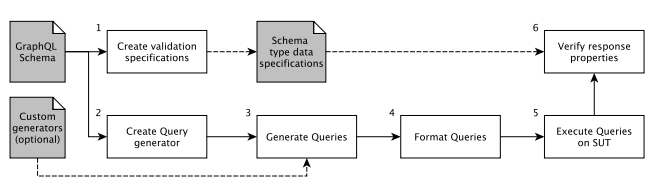
\includegraphics[width=\textwidth,height=\textheight,keepaspectratio]{content/einleitung/toolchain}
\end{center}

Verbesserungen in dieser Arbeit sind insbesondere in den Punkten 2 und 6 (6 wenn genug Zeit) geplant.

\begin{description}
    \item[Create Query Generator (Punkt 2)] Kapitel Testgenerierung
    \item[Verify response properties (Punkt 6)] Kapitel Testauswertung
\end{description}

\subsection{Testgenerierung}

Der bisherige Ansatz der Testgenerierung ist eine zufallsbasierte Suche.
Hierbei wird ein GraphQL-Schema geladen und nach dem Query-Type gefragt.
Der Query-Type definiert alle erlaubten Anfragen an die API.
Das Ergebnis einer jeden Anfrage ist (ein Knoten) / (eine Liste von Knoten).
Jeder Knoten kann dann verwandte Knoten haben.
Eben diese werden dann mit zufallsbasierter Suche abgefragt, jedoch nur bis zu einer bestimmten Pfadlänge die
durch das Rekursionslimit festgelegt ist, eben um unendliche Suchräume zu vermeiden.
Nun ist offensichtlich, dass es durchaus auch Pfade geben kann, die länger
als das Rekursionslimit sind und somit nicht vom Testtool berücksichtig werden.
Im Sinne einer guten Testcoverage wollen wir aber möglichst
jede Funktion mit Tests überdecken, somit erreicht die bisherige Methode leider nicht eine zufriedenstellende Lösung im Sinne
der Testcoverage.
Diese Arbeit soll die bisherige Methode verbessern indem Schritt 2, der Query-Generator, verbessert wird mit einem
endlichen Algorithmus der Graphen jeder Größe und Struktur zuverlässig abdeckt. Hierfür müssen verschiedene Überdeckungskriterien
erst definiert werden, allerdings sei schon zu sagen, die hier vorgestellte Methode hat als Ziel, das jede Kante und jeder
Knoten des Graphens hierdurch mit mindestens einem Test abgedeckt werden, sodass wir eine erhebliche Verbesserung in der
Zuverlässigkeit der Testcoverage erlangen.

\subsection{Testauswertung}


Die Auswertung der Tests nach " Automatic Property-based Testing of GraphQL-API's " erfolgt durch einen Typabgleich von Query und Response.
Eine Validierung der Response wird zeitgleich mit dem erstellen der Querys erledigt. Hierdurch folgt die Limitierung, dass das Testtool
aus dem GraphQL-Schema wissen kann, welchen Typ eine Antwort hat, allerdings ist nicht erschließbar, welche genauen Attribute eine Rückgabe hat.
So kann eine Anfrage, die als Typ \verb+Automarke+ hat, jede Automarke akzeptieren.
Sähe die Anfrage allerdings so aus: \verb+getMarke("Opel Corsa")+ und die Antwort \verb+Marke(name:Audi)+ dann wäre hier eigentlich
ein Fehler, das Testtool würde aber akzeptieren, da die Typzuordnung zutreffend ist.
Es wäre besser, wenn das Testtool nicht nur den Typ der Response auswertet sondern auch ihren Inhalt.
Ob dies umgesetzt wird in dieser Arbeit wird sich zeigen (Zeitliche Komponente; TODO)
\newpage

\section{Umsetzung}

Zuallererst wird in dieser Arbeit etwas Theorie definiert und in Bezug gesetzt. Angefangen mit einer allgemeinen Definition
eines Graphens im mathematischen Sinne und GraphQL als Schnittstelle, wird dann ein Bezug dieser beiden Themen
zueinander hergestellt.
Im folgenden wird erklärt, was Software-Testing überhaupt ist und inwiefern dieses mit Graphen zusammenhängt.
Hierfür werden insbesondere Graphüberdeckungen betrachtet.
Abschließend für den Theorie-Teil folgt eine Erklärung wie Graphüberdeckungskriterien und Algorithmen die diese Kriterien
erfüllen können, helfen können um GraphQL-APIs zu testen.
Um diese theoretischen Erkenntnisse zu validieren und die eingängliche Behauptung zu beweisen wird dann eine Implementierung
des PrimePath Algorithmus erstellt die dann den Query-Generator vom Paper " Automatic Property-based Testing of GraphQL-API's " ersetzen soll.
Hierbei ist das Ziel, große Teile des bestehenden Codes zu nutzen und den Query-Generator nathlos in das Programm einzubinden, sodass
gezeigt werden kann, dass unsere hier erarbeitete Methode funktioniert.
Um zu beweisen, dass unsere Methode funktioniert folgt ein Vergleich beider Generierungsalgorithmen.
Verschiedene Metriken sind hierbei interessant, insbesondere jedoch die Anzahl der generierten Tests, die Dauer
der Berechnung aller Tests und die Coverage des Graphens.
Insbesondere bei der Anzahl an generierten Test / Coverage erhoffen wir uns, dass durch weniger Tests eine höhere Coverage erreicht werden
kann. Außerdem erwarten wir, dass die Berechnungszeit für eine vollständige Coverage geringer sein sollte als bei der zufallsbasierten Suche.
Hierfür werden die Experimente an 3 verschiedenen GraphQL-API's ausgetestet, 2 stammen hiervon aus dem originalen Paper und eins wird
eigens für unsere Methode entwickelt um an diesem besonders die Limitierungen des ursprünglichen Tools zu zeigen und die Lösung der Limitierungen zu validieren.






  % Hauptteil
  \chapter{related Work / ähnliche Arbeiten}

Da Software-Testing ein stetig wachsendes Thema ist und der allgemeine Konsens \"man kann nicht genug testen\" existiert ist
es klar, dass diverse Arbeiten in Richtung Testautomatisierung erstellt wurden. In diesem Abschnitt sollen ähnliche Arbeiten
genannt werden sowie Unterschiede zu diesen Arbeiten benannt werden.

\section{EvoMaster}

EvoMaster ist ein Open-Source Tool welches sich automatisiertes Testen von Rest-APIs und GraphQL APIs zur Aufgabe gemacht hat.
Aktuell kann durch EvoMaster sowohl WhiteBox Testing als auch BlackBox Testing durchgeführt werden jedoch ist ein
Whitebox Test mittels Vanilla-EvoMaster nur für Rest-APIs möglich die mit der JVM lauffähig sind.
Im Paper \"White-Box and Black-Box Fuzzing for GraphQL APIs" (Quelle hier) wurde ein System on-Top für EvoMaster
erstellt welches GraphQL Tests generieren kann. Hierbei soll sowohl WhiteBox als auch BlackBox Testing möglich sein.
Das erstellte Framework in diesem Paper arbeitet nach folgendem Prinzip:

\begin{center}
    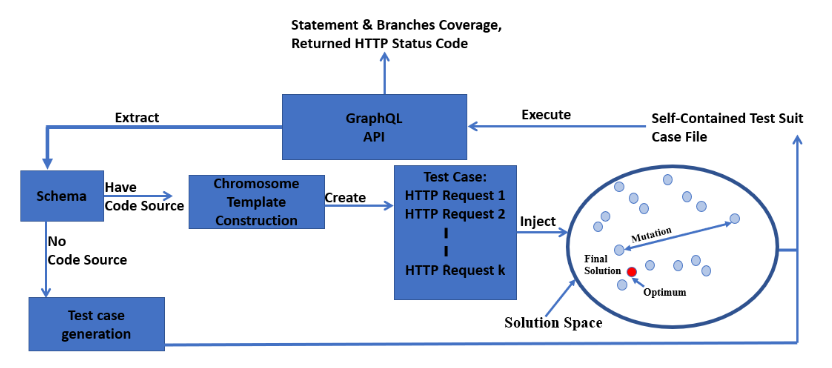
\includegraphics[width=\textwidth,height=\textheight,keepaspectratio]{content/hauptteil/related Work/evomaster_framework}
\end{center}

WhiteBox Testing ist möglich insofern Zugang zum GraphQL-Schema und zum Source Code der API gegeben ist. Andernfalls ist
nur BlackBox Testing möglich. Zur Testgenerierung wird ein genetischer Algorithmus genutzt welcher die Tests generiert.
Wie dieser genetische Algorithmus genau funktioniert kann im Paper selbst nachgelesen werden (hier Quelle).
Im Vergleich mit unserer geplanten Arbeit mittels des Prime-Path-Algorithmus ergeben sich einige Unterschiede, diese sind
unter anderem: Nutzung eines evolutionären Algorithmus Many-Independent-Objective (MIO).
Im Paper selbst wird davon ausgegangen, dass andere evolutionäre Algorithmen unter Umständen passender wären als der MIO Algorithmus
für die Testgenerierung. Jedoch ist ein evolutionärer Algorithmus auch immer ein stochastisch, heuristisch sich dem Optimum annähernder Algorithmus. (Beleg hierfür)
Im Gegensatz dazu ist der Ansatz dieser Arbeit ein natürlicher Algorithmus der beweisbar ideale Lösungen auf direkte Art bietet
und im ersten Durchlauf direkt sein ideales Ergebnis ermittelt. Die ideale Lösung bezieht sich hierbei auf bestimmte
Code-Coverage Kriterien die durch unseren Algorithmus erfüllt werden.  Inwiefern der evolutionäre Algorithmus diese
Kriterien erfüllt bleibt offen, es ist jedoch davon auszugehen, dass er sich einer idealen Lösung dieser Kriterien nur
annähert da er eben ein stochastischer Algorithmus ist. (beleg oder Quelle)

\section{Deviation Testing}

Da GraphQL dynamisch auf Anfragen reagiert und es somit möglich ist, in seiner Anfrage einzelne Felder mit einzubeziehen
oder auch auszuschließen ist dies im Grunde genommen ein einzelner Test-Case.
Im Paper \" Deviation Testing: A Test Case Generation Technique for GraphQL APIs" wird diese Gegebenheit benutzt und
aus einer selbstdefinierten Query werden hier einzelne Test-Cases gebildet. Ein solcher Test macht je nach Implementierung
der GraphQL-Resolver druchaus Sinn, da im Backend Felder durchaus zusammenhängen können und es Bugs geben kann wenn
Resolver fehlerhaft definiert sind. z.B. könnte folgende Definition zu solchen Fehlern führen:

(hier BSP mit Code einfügen)

Da Deviation Testing jedoch nur bestehende Tests erweitert um mögliche Felder mitzutesten werden hier keine neuen Tests generiert.
Durch Deviation Testing werden bestehende Tests nur erweitert allerdings muss eine Edge-Coverage gegeben sein damit diese Arbeit
ein zufriedenstellendes Ergebnis erzeugt. Eine Edge-Coverage in einem komplexen Graphen ist allerdings sehr wahrscheinlich
schwer umsetzbar mit manuellem Test schreiben. Eine Paarung von Edge-Coverage mit Deviation-Testing wäre sicherlich Interessant.
Genau so wäre es interessant Deviation Testing als Teil unserer Arbeit zu nutzen indem mit diesem Tool die Tests erweitert werden.
(initialer Plan war es, einfach immer alle Felder eines Nodes zu testen, hierdurch wäre es möglich auch alle Varianten noch zu testen)

\section{AutoGraphQL}

Klassisches Testen von Anwendungen beeinhaltet, dass möglichst das komplette System getestet wird bevor es verwendet wird.
Im Paper "Harvesting Production GraphQL Queries to Detect Schema Faults" wird ein gänzlich anderer Ansatz verfolgt.
Hierbei ist es nicht wichtig die gesamte GraphQL-API vor der Veröffentlichung zu testen sondern
echte Queries die in Production ausgeführt werden zu sammeln.
Der Ansatz der hierbei verfolgt wird begründet sich daraus,
dass ein Testraum für GraphQL potentiell unendlich sein kann und es sehr wahrscheinlich ist, dass nur ein kleiner
Teil der API wirklich intensiv genutzt wird, sodass auch nur dieser Teil wirklich stark durch Tests abgedeckt werden muss.
AutoGraphQL läuft hierbei in zwei Phasen wobei in der ersten Phase alle einzigartigen Anfragen geloggt werden.
In der zweiten Phase werden dann aus den geloggten Anfragen Tests generiert.
Hierbei wird für jede geloggte Query genau ein Test-Case erstellt.
Bei dieser Art des Testens wird insbesondere darauf Wert gelegt, dass es keine Fehler im GraphQL Schema gibt.
Dies ist ein wichtiger Teil um GraphQL-API's zu testen allerdings noch kein vollständiger Test denn hier wird außer Acht gelassen,
dass eine Query konform zum GraphQL-Schema sein kann aber trotzdem falsch indem zum Beispiel falsche Daten zurückgegeben werden
durch falsche Referenzierung oder ähnlichem.
In dem zu entwickelndem Tool sollten alle Querys die von AutoGraphQL geloggt werden auch berücksichtig werden da sie durch
den Prime-Path Algorithmus auch ermittelt werden.
Es kann allerdings sinnvoll sein AutoGraphQL als Monitoring-Software mitlaufen zu lassen und weitere etwaige Fehler hiermit zu loggen
und automatisch daraus Test-Cases erstellen zu können damit zukünftig keine Fehler dieser Art mehr passieren.




  \chapter{Grundlagen}
\label{theorie}

Das automatisierte Testen von GraphQL-APIs erfordert ein spezifisches Domänenwissen in verschiedenen Teilbereichen der
Informatik und Mathematik, insbesondere die Graphentheorie und das Softwaretesten.
Dieses Domänenwissen wird in den folgenden Abschnitten auf Grundlage von zwei Lehrbüchern~\cite{software-testing,graphentheorie} erarbeitet
und in Kontext gesetzt.
Die Graphentheorie wird benötigt, um die Struktur von GraphQL auf einer abstrakten Ebene besser verstehen zu können.
Außerdem setzen die in~\cite{software-testing} vorgestellten Überdeckungskriterien ein grundlegendes Wissen über Graphentheorie und Softwaretests voraus.
  \section{Graphentheorie}
\label{sec:graphentheorie}

Da GraphQL es ermöglicht, dass komplexe Beziehungen innerhalb eines Datenmodells in Form von Graphen modelliert werden~\cite[vgl. Modelling with Graph(QL)]{graphqlgraphtheory}
benötigt man die Graphentheorie, da diese Methoden liefert, um Graphen zu definieren und zu analysieren.
Des Weiteren sind die Testabdeckungskriterien, die später genutzt werden, eng mit der Graphentheorie verbunden.
Die folgenden Absätze werden eher theoretisch gehalten.
Die Zusammenhänge zwischen der Graphentheorie und Testen von GraphQL-APIs werden sich jedoch später erschließen.

\subsection{Ungerichteter Graph}

Ein Graph ist ein mathematisches Modell.
Es kann dazu verwendet werden, Beziehungen zwischen Objekten darzustellen.
Nach~\cite{graphentheorie} ist ein ungerichteter Graph wie folgt definiert:

\begin{definition}
    Ein ungerichteter Graph ist ein Paar $\textrm{G = (V, E)}$ zweier disjunkter Mengen mit \\ E $\subseteq$ V^2
    \label{graphdef}
\end{definition}\cite[vgl. S.2 0.1 Graphen]{graphentheorie}
\\
\\
Die Elemente der Menge $V$ heißen Knoten (Vertices).
Verbindungen zwischen den Knoten sind Elemente der Menge $E$ und diese nennt man Kanten (Edges).
In dieser Definition spielt die Ordnung der Elemente von E keine Rolle, daher nennt man solche Graphen auch ungerichtete Graphen.
Um Graphen darzustellen, gibt es verschiedene Ansätze.
Der geläufigste Ansatz ist es, Knoten als Punkte und Kanten als Verbindungslinien zu zeichnen.
Häufig wird auch eine Adjazenzmatrix genutzt, bei dieser wird mit $0,1$ aufgeschlüsselt, welche Knoten eine Verbindung haben.
Bei $0$ existiert keine Kante zwischen den Knoten und bei $1$ existiert eine.

\begin{example}
    Ein Graph sei definiert mit $V = \{ 1, 2, 3 \}$ und $E = \{(1,1), (1,2), (1,3) \}$ \\
    Mögliche Darstellungen des Graphen sind in Abbildung~\ref{zeichnung} und~\ref{adjam} gezeigt.
    \label{exmgr}
\end{example}
    \begin{figure}[h!]
        \centering
        % Linke Seite: Code
        \begin{minipage}{0.45\textwidth}
            \centering
            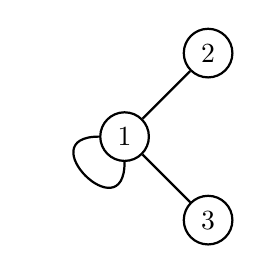
\begin{tikzpicture}[node distance={15mm}, thick, main/.style = {draw, circle}]
                \node[main] (1) {$1$};
                \node[main] (2) [above right of=1] {$2$};
                \node[main] (3) [below right of=1] {$3$};
                \draw (1) to [out=180,in=270,looseness=5] (1);
                \draw (1) -- (2);
                \draw (1) -- (3);
            \end{tikzpicture}
            \caption{Gezeichneter Graph}
            \label{zeichnung}
        \end{minipage}
        \hfill
        \begin{minipage}{0.45\textwidth}
            \centering
            \begin{array}{c|ccc}
                & 1 & 2 & 3 \\
                \hline
                1 & 1 & 1 & 1 \\
                2 & 0 & 0 & 0 \\
                3 & 0 & 0 & 0 \\
            \end{array}
            \caption{Adjazenzmatrix}
            \label{adjam}
        \end{minipage}
    \end{figure}

\subsection{Gerichteter Graph}

Gerichtete Graphen sind die Grundlage vieler Überdeckungskriterien~\cite[vgl. 2.1 Overview]{software-testing}.
Daher werden sie hier definiert.

\begin{definition}
    Ein gerichteter Graph ist ein Paar $\textrm{G = (V, E)}$ zweier disjunkter Mengen mit zwei Funktionen
    init: E \textrightarrow V und ter: E \textrightarrow V, die jeder Kante e eine Anfangsecke init(e) und eine
    Endecke ter(e) zuordnen~\cite[S.26 0.10 Verwandte Begriffsbildungen]{graphentheorie}.
    \label{gerichtetergraphdef}
\end{definition}

Bei einem gerichteten Graphen ist die Sortierung der Kantenpaare wichtig.
Die Funktionen $init$ und $ter$ können nämlich am einfachsten durch die Sortierung der Elemente eines Kantenpaares umgesetzt werden.
Hierbei ist das erste Element des Kantenpaares die Anfangsecke und das zweite Element ist die Endecke.
Die Kanten in einem gerichteten Graphen werden mit einem Pfeil gezeichnet.
Dabei zeigt der Pfeil stets in Richtung Endecke.
Der in Beispiel~\ref{exmgr} definierte Graph ist als gerichteter Graph in Abbildung~\ref{graphexample} gezeigt.

\begin{figure}
    \begin{center}
        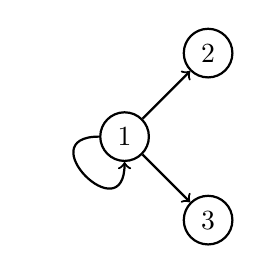
\begin{tikzpicture}[node distance={15mm}, thick, main/.style = {draw, circle}]
            \node[main] (1) {$1$};
            \node[main] (2) [above right of=1] {$2$};
            \node[main] (3) [below right of=1] {$3$};
            \draw[->] (1) to [out=180,in=270,looseness=5] (1);
            \draw[->] (1) -- (2);
            \draw[->] (1) -- (3);
        \end{tikzpicture}
    \end{center}
    \caption{ein gerichteter Graph}
    \label{graphexample}
\end{figure}

\subsection{Gewichteter Graph}

Für die spätere Entwicklung des Testentwurfs ist es wichtig, gewichtete Graphen zu definieren.
Zuvor wurde eine Kante in Definition~\ref{graphdef} und Definition~\ref{gerichtetergraphdef} als ein Tupel $(x, y)$ eingeführt.
Ein gewichteter Graph weist jeder Kante ein Kantengewicht zu, dies ist im Allgemeinen eine positive, reelle Zahl~\cite[vgl. S. 251]{graphentheorie3}.

\begin{definition}
    Ein Graph G = (V,E) mit einer Abbildung g : E \textrightarrow $\mathbb{R}_{>0}$ heißt gewichteter Graph.
    Die Abbildung g heißt Gewichtsfunktion. Für $e \in E$ heißt g(e) das Gewicht von e.
    Das Gewicht von G ist die Summer der Gewichte aller Kanten, g(G) = \sum_{e \in G} g(e).\\
    \cite[vgl.~Definition~6.1~S.~251]{graphentheorie3}
    \label{gewichtetergraph}
\end{definition}
\\
\\
Für spätere Anwendungszwecke muss die Definition jedoch ein wenig allgemeiner gefasst werden.
Die Felder eines GraphQL-Typens sollen später als Gewicht genutzt werden, um Tests zu entwerfen.
Um dies zu erleichtern, soll die Definition~\ref{gewichtetergraph} verallgemeinert werden durch eine Anpassung der Gewichtsfunktion.
Die neue Definition soll vorerst \textit{allgemein gewichteter Graph} genannt werden.

\begin{definition}
    Ein Graph G = (V,E) mit einer Abbildung g: E \textrightarrow X heißt allgemein gewichteter Graph.
    Die Menge X ist frei wählbar.
    \label{allgemeingewichtetergraph}
\end{definition}

\subsection{Pfad}

Ein Pfad, oft auch Weg genannt, ist eine Sequenz von Knoten, die nachfolgend durch Kanten miteinander verbunden sind~\cite[vgl. S. 7 0.3]{graphentheorie}.

\begin{definition}
    Ein Weg ist ein nicht leerer Graph P = (V,E) der Form $V = {x_{0}, x_{1}, ..., x_{k}}$ und $E = {x_{0}x_{1}, x_{1}x_{2}, \ldots, x_{k-1}x_{k}}$ wobei die $x_{i}$
    paarweise verschieden sind~\cite[vgl. S. 7]{graphentheorie}.
\end{definition}

Ein Weg wird oft durch die Folge seiner Knoten beschrieben also $P=x_{0} x_{1} \ldots x_{k}$ \cite[vgl. S.7]{graphentheorie}
Die Länge eines Weges ist die Anzahl der Kanten, die dieser besucht~\cite[vgl. S. 7]{graphentheorie}.
In gewichteten Graphen ist das Gewicht eines Pfads die Summe aller Gewichte der einbezogenen Kanten~\cite[vgl. 7.2 kürzeste Wege]{graphentheorie3}.

\begin{example}
    Es sei ein Graph G definiert mit V = $\{n1,n2,n3,n4,n5,n6,n7,n8\}$ und E = $\{(n1,n2),(n2,n3),(n3,n4),(n4,n1),(n2,n5),(n3,n6),(n5,n7),(n6,n8)\}$.
    Ein möglicher Pfad von Knoten $n1$ zu $n8$ ist der Pfad $p = \{(n1, n2), (n2, n3), (n3, n6), (n6, n8)\}$.
    Der Pfad p ist in Abbildung~\ref{pfadbsp} rot markiert \\ \\
\end{example}

\begin{figure}[H]
    \begin{center}
        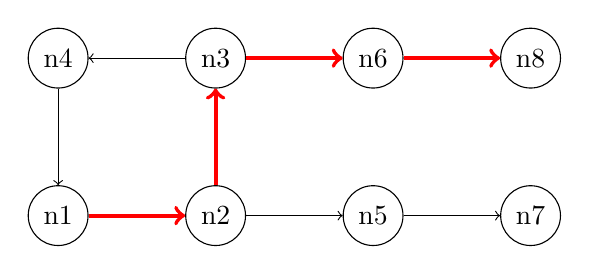
\begin{tikzpicture}
            \node[circle, draw] (n1) at (0,0) {n1};
            \node[circle, draw] (n2) at (2,0) {n2};
            \node[circle, draw] (n3) at (2,2) {n3};
            \node[circle, draw] (n4) at (0,2) {n4};
            \node[circle, draw] (n5) at (4,0) {n5};
            \node[circle, draw] (n6) at (4,2) {n6};
            \node[circle, draw] (n7) at (6,0) {n7};
            \node[circle, draw] (n8) at (6,2) {n8};

            \draw[->, red, line width=1.5pt] (n1) -- (n2);
            \draw[->, red, line width=1.5pt] (n2) -- (n3);
            \draw[->] (n3) -- (n4);
            \draw[->] (n4) -- (n1);
            \draw[->] (n2) -- (n5);
            \draw[->, red, line width=1.5pt] (n3) -- (n6);
            \draw[->] (n5) -- (n7);
            \draw[->, red, line width=1.5pt] (n6) -- (n8);
        \end{tikzpicture}
    \end{center}
    \caption{Pfad von n1 zu n8}
    \label{pfadbsp}
\end{figure}

\subsection{Kreis}

Ein Kreis in einem Graphen ist ein Weg, bei dem gilt: $Anfangsknoten = Endknoten$ \cite[vgl. S. 8]{graphentheorie}
Die Größe eines Kreises ist die Länge des Wegs, den dieser Kreis bildet.
Der kürzeste Kreis eines Graphens nennt sich $Tailenweite~g(G)$ und der längste Kreis ist der Umfang~\cite[vgl. S.8]{graphentheorie}.
Der Graph aus Beispiel~\ref{pfadbsp} hat einen Kreis der Länge 4 und ist in Abbildung~\ref{zyklgraph} rot eingezeichnet.

\begin{figure}[h!]
    \centering
    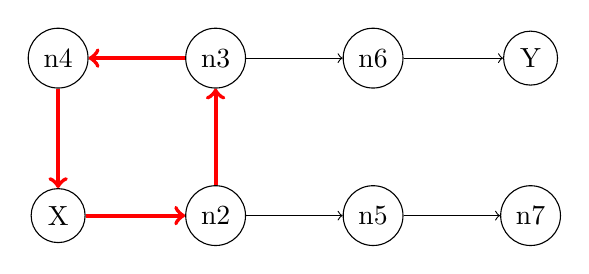
\begin{tikzpicture}
        \node[circle, draw] (n1) at (0,0) {X};
        \node[circle, draw] (n2) at (2,0) {n2};
        \node[circle, draw] (n3) at (2,2) {n3};
        \node[circle, draw] (n4) at (0,2) {n4};
        \node[circle, draw] (n5) at (4,0) {n5};
        \node[circle, draw] (n6) at (4,2) {n6};
        \node[circle, draw] (n7) at (6,0) {n7};
        \node[circle, draw] (n8) at (6,2) {Y};

        \draw[->, red, line width=1.5pt] (n1) -- (n2);
        \draw[->, red, line width=1.5pt] (n2) -- (n3);
        \draw[->, red, line width=1.5pt] (n3) -- (n4);
        \draw[->, red, line width=1.5pt] (n4) -- (n1);
        \draw[->] (n2) -- (n5);
        \draw[->] (n3) -- (n6);
        \draw[->] (n5) -- (n7);
        \draw[->] (n6) -- (n8);
    \end{tikzpicture}
    \caption{Ein zyklischer Graph}
    \label{zyklgraph}
\end{figure}

Im Kontext des Testentwurfs sind Kreise besonders interessant, da diese für einen potenziell unendlich großen Testraum sorgen.
In einem azyklischen gerichteten Graphen, also einem gerichteten Graphen, der keinen Kreis besitzt, ist die Menge aller möglichen Pfade endlich.
Bei einem Graphen mit Zyklen ist die Menge aller möglichen Pfade unendlich.
Dies folgt aus der Tatsache, dass jeder Pfad, der den Kreis beinhaltet, diesen Kreis ein weiteres Mal ablaufen kann und somit stets ein neuer Pfad generiert wird.

\newpage
  \section{GraphQL}

GraphQL ist eine Open-Source Query-Language (Abfragesprache) und Laufzeitumgebung die von Facebook entwickelt wurde. (vgl. GraphQL-Spec)
Die Besonderheiten von GraphQL sind, dass man mit nur einer einzelnen Anfrage mehrere Ressourcen gleichzeitig abfragen kann und die
Daten in diesem Schema stark durch einen Typgraphen definiert sind. So lässt sich einerseits die Effizienz stark erhöhen indem weniger Anfragen
gestellt werden die zeitgleich eine höhere Informationsdichte haben.
Außerdem erleichtert GraphQL die Kommunikation von Schnittstellen indem die geünschten Felder schon in der Query definiert werden
und direkt den erwarteten Datentyp zusichern.
Hier liegt auch der große Vorteil im Vergleich zum direkten technologischen Konkurenten REST API.
Bei REST-APIs sind nämlich für verschiedene Ressourcen auch jeweils eine eigene Anfrage nötig und die Typsicherheit ist nicht so stark gegeben
wie bei GraphQL-APIs.
Diese beiden großen Vorteile sorgen dafür, dass GraphQL an Popularität gewinnt und zunehmend eingesetzt wird.
Im Kontext dieser Arbeit ist ein tiefgreifendes, technologisches Verständniss von GraphQL essentiell, deshalb wird hier
eine tiefgreifende Erklärung von GraphQL folgen.

\subsection{Schema \& Typen}

Grundlage einer jeden GraphQL-API ist ein GraphQL-Schema.
Dieses Schema definiert genau wie die Daten der API aufgebaut sind und welche Informationen exisitieren.
Ein GraphQL-Schema ist eine Sammlung von Typen.
Typen sind Objekte einer Datenstruktur.
Ein Typ definiert alle Informationen über sich, hierbei wird für jede Information ein Feld angelegt.
Das Feld kann entweder ein Standarddatentyp wie String, Integer etc. sein oder ein anderer Typ.
Falls das Feld ein anderer Typ ist, so entspricht diese Beziehung einer Kante in einem Graphen.
Dies bedeuet, dass eine Abfrage dieses Feldes dann ein Objekt des Types zurückliefert und hier auch die gewünschten Felder
definiert werden müssen.
Ein sehr einfaches Schema wäre zum Beispiel die Beziehung zwischen Büchern und Authoren.
Ein Buch hat hierbei einen Titel und einen Author.
Ein Author hat einen Namen und ein Geburtsdatum.
Ein Schema für dieses Beispiel sähe wie folgt aus:

\begin{center}
    \begin{verbatim}
        type Buch {
            title: String
            author: Author
        }
        type Author{
            name: String
            geburtsdatum: Date
        }
    \end{verbatim}
\end{center}

Es lässt sich also festhalten, dass ein GraphQL-Typ immer als ein Tupel \verb+(Name, Felder)+ definiert wird wobei
die Felder eine Liste an Tupeln \verb+(Feldname, Feldtyp, Datentyp)+ sind.
Hierbei gelten folgende Einschränkungen für die Elemente des Tupels:

\begin{center}
    \begin{itemize}
        \item[Feldname] ein eindeutiger Feldbezeichner
        \item[Feldtyp] gibt Einschänkungen vor, z.B. nicht Null (durch \verb+!+), Listentyp (durch \verb+[]+) etc.
        \item[Datentyp] der explizite Typ den das Feld hat, kann Standarddatentyp oder anders definierter Type sein
    \end{itemize}
\end{center}

Wenn ein Typ ein Feld enthält, das kein Standarddatentyp ist so entspricht dieses Feld einer Kante in einem Graphen.
Dieses Feld muss dann in einer Query näher definiert werden indem angegeben wird, welche Felder nun vom Typ zu dem die
Kante führt, ausgegeben werden sollen.

\subsection{vordefinierte Typen}

Jedes GraphQL-Schema definiert intial mehrere Typen die spezielle Aufgaben haben und nicht vom User überschrieben werden können.
Im folgenden werden wir auf einige wichtige dieser Typen eingehen.

\subsubsection{Scalar-Types}

Grundlegende Datentypen (Standarddatentypen) werden durch Scalar Types ausgedrückt. Scalar-Types repräsentieren einzelne Werte
wie z.B. einen Integer, einen String, Boolean Werte oder auch Datumstypen.
Ein Scalar-Type kann nicht vom User geändert werden und enthält auch keine anderen Typen (im Gegensatz zu Objekttypen die das können).
Es ist möglich auch eigene Scalar-Types festzulegen jedoch sind in der offiziellen Spezifikation von GraphQL
lediglich folgende Scalar-Types definiert:

\begin{center}
    \begin{itemize}
        \item[Int] 32-bit Integer
        \item[Float] Gleitkommazahl nach IEEE 754
        \item[String] frei wählbarer Text (leerer String zählt nich als non-Null!)
        \item[Boolean] True;False repräsentiert durch internen boolean-type. Ansonsten 0 & 1
        \item[ID] einzigartiger Identifier, intern behandelt wie ein String
        \item[Scalar Extensions] Rohkonstrukt von dem geerbt werden kann für eigen definierte Typen
    \end{itemize}
    (vgl. GraphQL-Sepzifikation 3.5)
\end{center}

\subsubsection{Query-Type}

Der Query-Type definiert alle erlaubten Anfragen (Leseoperationen) an die GraphQL-API.
Hierbei können Anfragen mit und ohne Eingabeparameter angegeben werden.
Die definierten Anfragen haben, wie jeder Typ, einen eindeutigen Bezeichner, welcher dann auch in der zustellenden Query
benutzt wird.
Die Felder der Antwort hängen hierbei vom Feldtypen ab. Ist das Ergebnis der Query-Definition ein Standarddatentyp, so wird
es direkt ausgegeben. Ist es ein anderer definierter Typ, so müss näher bestimmt werden welche Felder erwartet werden.
Nutzen wir das Beispiel der Bücher & Autoren weiter, könnte man wie folgt einen Query-Type definieren:

\begin{verbatim}
    type Query{
        # returns a List of all Books
        getBooks: [Book]
        # returns one random Book
        getBook: Book
        # returns the Author from a Book Title
        getBookByTitle(String title): Author
    }
\end{verbatim}


\subsubsection{Mutation}

Der Mutation-Type ist das Pendant des Query-Types. Im Mutation-Type werden alle erlaubten Schreiboperationen definiert.
Dies beeinhaltet das Erstellen, Aktualisieren und Löschen von Daten in der GraphQL-API.
Felder im Mutation-Type haben auch immer einen Rückgabewert, Konvention ist es hierbei, die veränderten Objekte zurückzugeben,
sodass der Client als Validierung exakt das Objekt bekommt, welches er sich "gewünscht hat".
Die Operationen die mittels Mutation hervorgerufen werden, werden linear abgearbeitet. So ist es in GraphQL möglich, die
Operationen miteinander zu verknüpfen. Man stelle sich z.B. vor, dass ein User seine Mail ändern will und gleichzeitig noch
seinen Namen. Mit REST wären hier zwei Anfragen nötig, GraphQL kann dies mit einer Anfrage erledigen.
Kehren wir wieder auf unser bisheriges Beispiel zurück, ein Mutationstyp hierfür könnte wie folgt aussehen:

\begin{verbatim}
    type Mutation{
        # erstelle einen Author

        # erstelle ein Buch

        # ändere den Titel eines Buches

        # ändere den Geburtstag eines Autors

    }
\end{verbatim}

eine einzelne Mutation kann Pflichtfelder und optionale Felder markieren.
Pflichtfelder werden mit einem ! markiert. Diese Felder müssen dann bei jeder Ausführung mitgesendet werden.
Optionale Felder benötigen dies nicht.







\subsubsection{Subscription}



\subsection{Resolver}

Bisher wurde sich vorallem mit der Strukturierung & Typisierung der Objekte in GraphQL beschäftigt.
Es fehlt noch die Funktionsweise

  \section{Zusammenhang Graphentheorie und GraphQL}

GraphQL erlaubt es uns, Typen zu definieren. Ein Type beinhaltet immer mindestens eine Property. Ein Type kann mit einem
Knoten eines Graphens gleichgesetzt werden. Und eine Beziehung zwischen Types als Kante. Hierdurch lässt sich dann
ein Typgraph entwickeln der als Bauplan für reale Graphen dient.
Man nehme zum Beispiel ein Buch und definiere hierfür einen Type

\begin{center}
    \begin{verbatim}
        type Book {
            id: Int
            title: String
        }
    \end{verbatim}
\end{center}

Es exisitiert jetzt ein Objekt Book mit den Eigenschaften id als Integer und title als String.
Repräsentiert als Graphen hätten wir nun einen einfachen Knoten der zwei Datentypen speichert.

\begin{figure}[!htbp]
    \begin{center}
        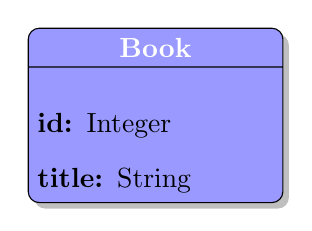
\begin{tikzpicture}
            \node (1)[abstract, rectangle split, rectangle split parts=2] at (4,8)
                {
                    \textbf{Book}
                    \nodepart{second} \begin{description}
                                          \item[id:] Integer
                                          \item[title:] String
                                      \end{description}
                };
        \end{tikzpicture}
    \caption{Graph mit 1 Type}
    \end{center}
    \label{fig:1type}
\end{figure}

Ein Objekt enthält 1 bis n Propertys. Diese Property kann entweder ein Standarddatentyp sein oder auf einen Type verweisen,
dies kann der eigene Type oder auch ein anderer Type sein.
Fügen wir unserem Beispiel des Buches eine Property hinzu mit dem Type Author wobei der Author selbst
wie folgt definiert wird:

\begin{center}
    \begin{verbatim}
        type Book {
            id: Int
            title: String
            author: Author
        }
        type Author {
            id: Int
            name: String
        }
    \end{verbatim}
\end{center}

So fügen wir unserem Graphen einen zusätzlichen Knoten hinzu
Die Beziehung zwischen dem Buch und Author wird durch eine gerichtete Kante zwischen dem Buch und dem Author dargestellt.
Hierdurch ergibt sich folgender Graph:

\begin{figure}
    \begin{center}
        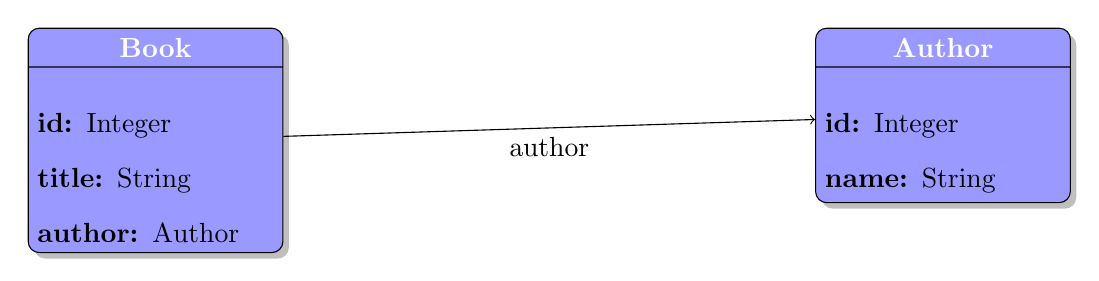
\begin{tikzpicture}
            \node (1)[abstract, rectangle split, rectangle split parts=2] at (0,0)
                {
                \textbf{Book}
                \nodepart{second} \begin{description}
                                      \item[id:] Integer
                                      \item[title:] String
                                      \item[author:] Author
                \end{description}
                };
            \node (2)[abstract, rectangle split, rectangle split parts=2] at (10,0)
                {
                \textbf{Author}
                \nodepart{second} \begin{description}
                                      \item[id:] Integer
                                      \item[name:] String
                \end{description}
                };
            \draw [->] (1) to node [midway,below]{author} (2);
        \end{tikzpicture}
    \end{center}
    \label{fig:2types}
\end{figure}

Fügen wir dem Author nun auch noch die Property written hinzu, so ergibt sich ein Kreis in diesem Graph.

\begin{verbatim}
    type Book {
        id: Int
        title: String
        author: Author
    }
    type Author {
        id: Int
        name: String
        written: [Books!]
    }
\end{verbatim}

so ergibt sich, dass wir einen zirkulären Graphen haben mit folgender Struktur

\begin{center}
    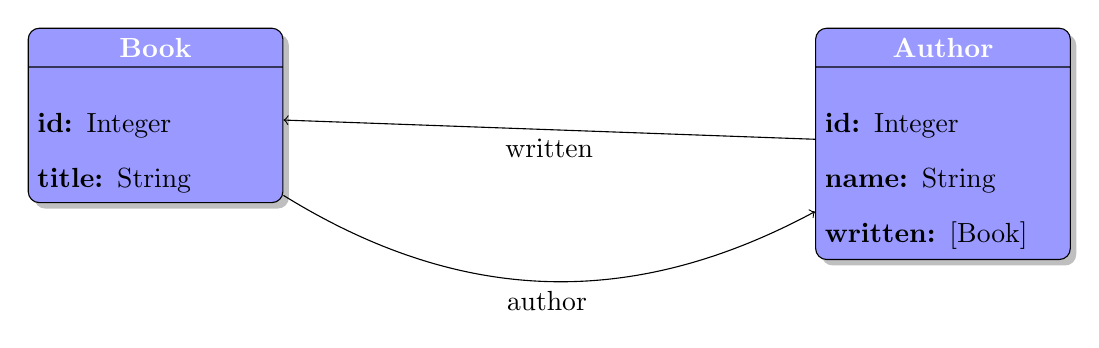
\begin{tikzpicture}
        \node (1)[abstract, rectangle split, rectangle split parts=2] at (0,0)
                {
                \textbf{Book}
                \nodepart{second} \begin{description}
                                      \item[id:] Integer
                                      \item[title:] String
                \end{description}
            };
            \node (2)[abstract, rectangle split, rectangle split parts=2] at (10,0)
                {
                \textbf{Author}
                \nodepart{second} \begin{description}
                                      \item[id:] Integer
                                      \item[name:] String
                                      \item[written:] [Book]
                \end{description}
            };

            \draw [ -> ] (1) to [bend right] node [midway,below]{ author } (2);
            \draw [ -> ] (2) to node [midway,below]{written} (1);
    \end{tikzpicture}
\end{center}


Dieses Schema ist ein Bauplan für einen sehr einfachen, zirkulären Graphen der durch GraphQL abgebildet wird.
In Realität können die Graphstrukturen die aus diesem Bauplan resultieren sehr unterschiedlich sein.
Für dieses Beispiel kann das bedeuten, dass folgende beide Graphen korrekt definierte Graphen sind jedoch komplett
andere Möglichkeiten bieten wie man sie abfragen kann. Hierdurch resultiert auch, dass die Abfragen
diverse Möglichkeiten haben je nach den unterliegenden Daten.

\begin{figure}
    \begin{center}
        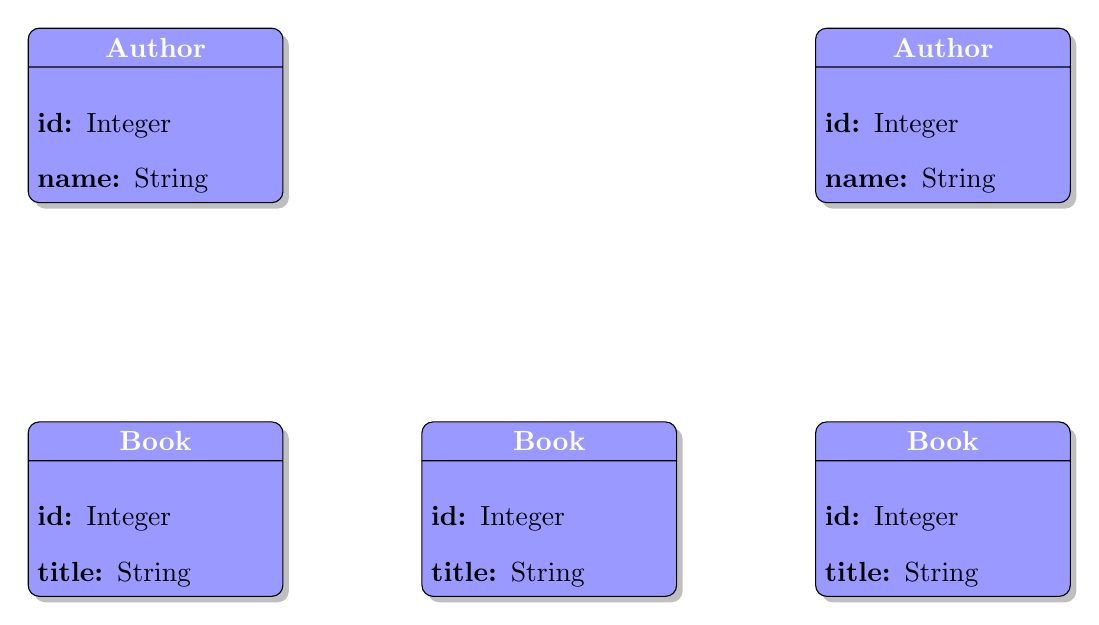
\begin{tikzpicture}
            \node (1)[abstract, rectangle split, rectangle split parts=2] at (0,0)
                {
                \textbf{Book}
                \nodepart{second} \begin{description}
                                      \item[id:] Integer
                                      \item[title:] String
                \end{description}
            };
            \node (2)[abstract, rectangle split, rectangle split parts=2] at (5,0)
                {
                \textbf{Book}
                \nodepart{second} \begin{description}
                                      \item[id:] Integer
                                      \item[title:] String
                \end{description}
            };
            \node (3)[abstract, rectangle split, rectangle split parts=2] at (10,0)
                {
                \textbf{Book}
                \nodepart{second} \begin{description}
                                      \item[id:] Integer
                                      \item[title:] String
                \end{description}
            };
            \node (4)[abstract, rectangle split, rectangle split parts=2] at (0,5)
                {
                \textbf{Author}
                \nodepart{second} \begin{description}
                                      \item[id:] Integer
                                      \item[name:] String
                \end{description}
            };
            \node (5)[abstract, rectangle split, rectangle split parts=2] at (10,5)
                {
                \textbf{Author}
                \nodepart{second} \begin{description}
                                      \item[id:] Integer
                                      \item[name:] String
                \end{description}
            };
        \end{tikzpicture}
    \caption{3 Bücher, 2 Autoren}
    \end{center}
\end{figure}


\begin{figure}
    \begin{center}
        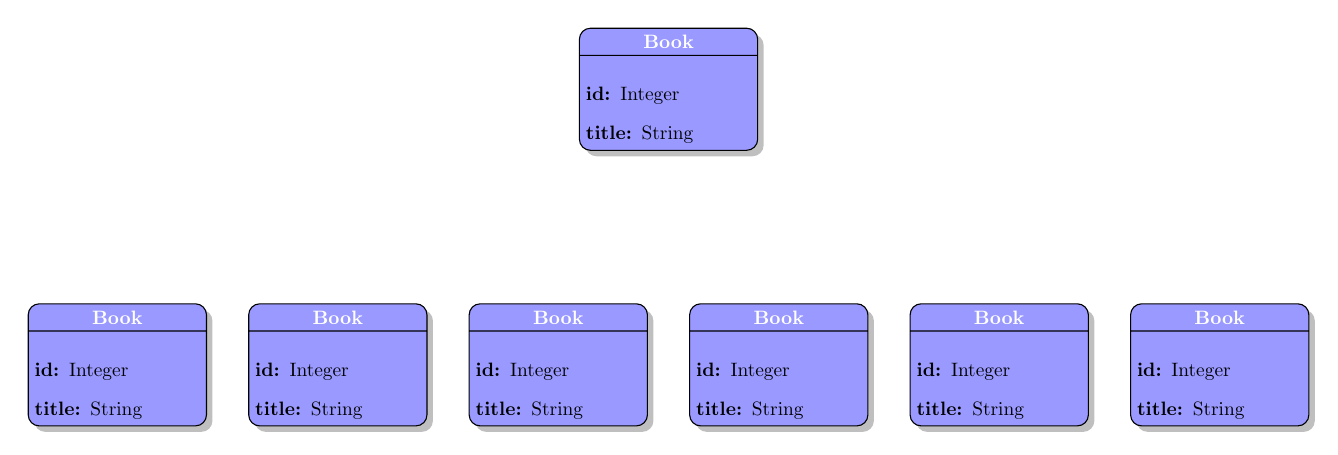
\begin{tikzpicture}[scale=0.7, transform shape]
            \node (1)[abstract, rectangle split, rectangle split parts=2] at (0,0)
                {
                \textbf{Book}
                \nodepart{second} \begin{description}
                                      \item[id:] Integer
                                      \item[title:] String
                \end{description}
            };
            \node (2)[abstract, rectangle split, rectangle split parts=2] at (4,0)
                {
                \textbf{Book}
                \nodepart{second} \begin{description}
                                      \item[id:] Integer
                                      \item[title:] String
                \end{description}
            };
            \node (3)[abstract, rectangle split, rectangle split parts=2] at (8,0)
                {
                \textbf{Book}
                \nodepart{second} \begin{description}
                                      \item[id:] Integer
                                      \item[title:] String
                \end{description}
            };
            \node (4)[abstract, rectangle split, rectangle split parts=2] at (12,0)
                {
                \textbf{Book}
                \nodepart{second} \begin{description}
                                      \item[id:] Integer
                                      \item[title:] String
                \end{description}
            };
            \node (5)[abstract, rectangle split, rectangle split parts=2] at (16,0)
                {
                \textbf{Book}
                \nodepart{second} \begin{description}
                                      \item[id:] Integer
                                      \item[title:] String
                \end{description}
            };
            \node (6)[abstract, rectangle split, rectangle split parts=2] at (20,0)
                {
                \textbf{Book}
                \nodepart{second} \begin{description}
                                      \item[id:] Integer
                                      \item[title:] String
                \end{description}
            };
            \node (7)[abstract, rectangle split, rectangle split parts=2] at (10,5)
                {
                \textbf{Book}
                \nodepart{second} \begin{description}
                                      \item[id:] Integer
                                      \item[title:] String
                \end{description}
            };
        \end{tikzpicture}
        \caption{6 Bücher, 1 Autor}
    \end{center}
\end{figure}

Definiert man nun, dass es zum Beispiel die StandardQuery "getBookAuthor(id): Author" geben soll. So bedeutet dies,
dass ein Author eines Buches abgefragt werden soll aufgrund der Id eines Buches.

(Hier Graphen einfügen mit Highlight der gewählten Knoten)




  \section{Testen}
\label{test}

Indem technische Geräte und somit auch Software im umfangreichen Maßstab Einzug nehmen in nahezu alle Bereiche des
Lebens ist es wichtig die Sicherheit, Qualität und Zuverlässigkeit von Software sicherzustellen. \cite[vgl. Introduction]{software-testing}
Um all dies sicherzustellen sind systematische Tests von Software nötig.
Ziel ist es sicherzustellen, dass die Software den definierten Anforderungen und Spezifikation entspricht.
Hierbei werden diverse Techniken und Ansätze verfolgt, die im folgenden kurz vorgestellt werden.

\subsection{Typen von Tests}

Es gibt verschiedene Sichtweisen auf das zu testende System.
Die Sichtweisen können intern oder extern bestimmt sein.
So sind Faktoren wie möglicher Zugriff auf Quellcode oder Architekturdetails des Systems essenziell wichtig um
zu entscheiden, welche Art von Tests angewandt werden.
Es gibt zwei generelle Sichtweisen und eine Mischform.
Das zu testende System wird als Box betrachtet.
Diese Box kann aus verschiedenen Sichten gesehen werden, die wir im Folgenden näher erläutern.
Die Ansätze unterscheiden sich vor allem in den zur Verfügung stehenden Informationen über das System.

\subsubsection{White-Box Testing}

Im WhiteBox-Testing stehen alle Informationen über das System zur Verfügung~\cite[vgl. 1.4.2 Code-Based Testing]{software-testing-craftmans}.
Der Tester hat Zugriff auf Code, Architekturdetails und besitzt Kenntnisse über alle möglichen Details des Systems~\cite[vgl. 1.4.2 Code-Based Testing]{software-testing-craftmans}.
Somit kann der Tester auf alle möglichen Informationen über das System zugreifen und damit seine Tests generieren.
Die erstellten Tests fundieren dann auf einem soliden Niveau, dass begründet wird durch das Domänenwissen über das System.
Verschiedene Techniken zur Analyse des Domänenwissens wurden entwickelt um die Informationen für die Testentwicklung zu nutzen.
Wir werden anschließend in Kapitel~\ref{graphueberdeckung} eine dieser Techniken näher untersuchen.

\subsubsection{Black-Box Testing}

Im BlackBox-Testing hat der Tester keinen Zugriff auf interne Funktionsweisen der Software.
Schwerpunkt des Testens ist es, dass die Software das tut, was in den Anforderungen gefordert ist \cite[vgl. Specification-Based Testing]{software-testing-craftmans}.
Da der Quellcode nicht einsehbar ist muss man sich darauf verlassen, dass die Anforderungen treffend forumliert wurden \cite[vgl.]{testmanagment}.
Das BlackBox-Testing hat einen methodischen Bezug zu Property-based Testing~\cite{property-based-testing}.

\subsubsection{Grey-Box Testing}

Das Grey-Box Testing ist eine Mischform von White und BlackBox Tests~\cite[vgl.]{testmanagment}.
Es sind in dieser Sicht Teile der Software bekannt aber man hat keinen umfassenden Einblick wie im White-Box Testing.
Es werden funktionale als auch strukturelle Testansätze verfolgt, je nachdem wie viel Informationen über das System tatsächlich 
verfügbar sind~\cite[vgl.]{graybox}.
Das System wird aus der Sicht des Endbenutzers getestet~\cite[vgl.]{testmanagment}, jedoch mit zusätzlichem Wissen über Teile des internen Aufbaus.

\subsection{Arten von Tests}

Neben verschiedenen Transparenzen auf das zu testende System gibt es verschiedene Granularitätsebenen der Tests.
Tests können von abgeleitet werden von Anforderungen, Spezifikationen, Designartifikaten und dem Programmcode~\cite[vgl. 1.1.1 Testing Levels Based on Software Activity]{software-testing}
Dabei können verschiedene Level an Tests definiert werden, diese sind eng verbunden mit den Entwicklungsaktivitäten einer Software~\cite[vgl. 1.1.1]{software-testing}.

\begin{figure}[h!]
    \centering
    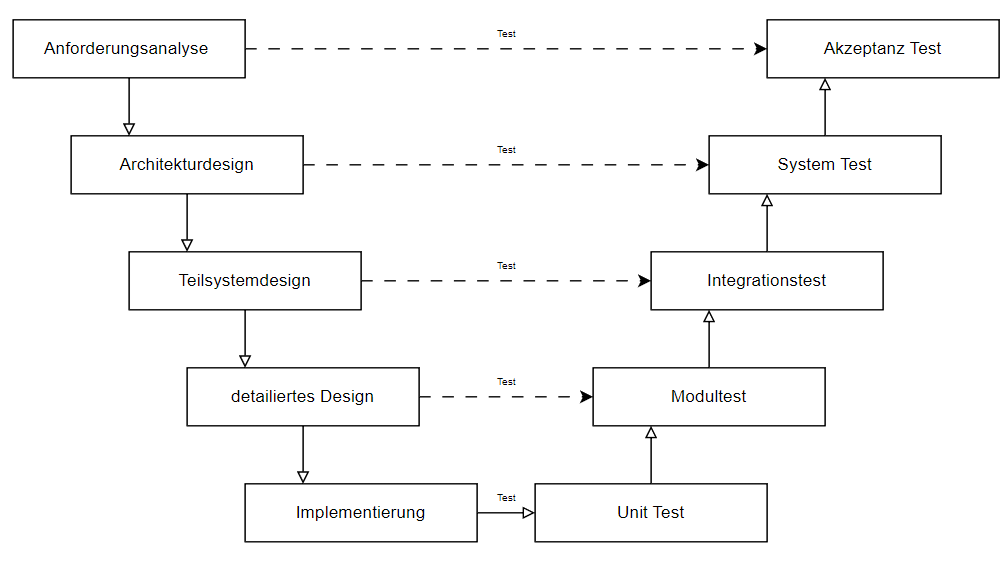
\includegraphics[width=\textwidth,height=\textheight,keepaspectratio]{img/vmodell}
    \caption{Softwareentwicklung und Test-Levels im V-Modell \cite[vgl. Figure 1.2]{software-testing}}
    \label{vmodelltest}
\end{figure}

Die verschiedenen Testebenen sollten schon im Designprozess Beachtung finden, denn die Formulierung von Test kann dabei helfen Designfehler zu finden
noch bevor die Software entwickelt wird~\cite[vgl. 1.1.1].
Die verschiedenen Ebenen der Tests spiegeln auch verschiedene Ansichten in den Tests wieder.
\newpage
\begin{figure}[h!]
    \begin{description}
        \item[Akeptanz Test] - Betrachten der Software hinsichtlich der Anforderungen
        \item[System Test] - Betrachten der Software hinsichtlich der Architektur
        \item[Integrationstest] - Betrachten der Software hinsichtlich der Teilsysteme
        \item[Modultest] - Betrachten der Software hinsichtlich detaiiliertem Design
        \item[Unit Test] - Betrachten der Software hinsichtlich konrekter Implementierung
    \end{description}\cite[vgl. 1.1.1]{software-testing}
\end{figure}

Im folgenden gehen wir noch einmal kurz auf jede einzelne Testebene etwas präziser ein.
Dabei ist die Reihenfolge von feingranular zu grobgranular.


\subsubsection{Unit Test}

Als feingranularste Testbene ist das Ziel des Unit-Testings den entwickelten Code zu testen.
Eine einzelne $Unit$ ist in Objekt-Orientierter Programmierung eine Funktion oder Methode~\cite[vgl. Unit Testing]{software-testing-craftmans}.
Ein einzelner Unit Test konzentriert sich dabei auf eine Funktion oder Methode.

\begin{figure}[h!]
    \begin{lstlisting}[language=Python]
        def add(a, b):
            return a + b
    \end{lstlisting}
    \caption{Eine einfache Python-Funktion}
    \label{unitfkt}
\end{figure}

\begin{figure}[h!]
    \begin{lstlisting}[language=Python]
    def test_add_positive():
        self.assertEqual(add(3, 5), 8)

    def test_add_negative():
        self.assertEqual(add(-3, -5), -8)

    def test_add_mixed():
        self.assertEqual(add(5, -3), 2)
    \end{lstlisting}
    \caption{Drei Unit Tests für die add-Funktion}
    \label{unitfkttest}
\end{figure}

Er prüft, ob die gegebene Einheit bei bekannten Eingaben die erwarteten Ausgaben liefert.
Für diese Tests werden häufig Testframeworks genutzt die bei der Entwicklung und Ausführung der Tests helfen~\cite{software-testing}.
In Abbildung~\ref{unitfkt} wurde eine Funktion defineirt und in Abbildung~\ref{unitfkttest} sind drei UnitTest mit PyTest~\cite{pytest} definiert.
Die Tests führen verschiedene Methoden aus und prüfen, dass das Ergebnis mit der Erwartung übereinstimmt.
Das $assertEqual$ übernimmt dabei die Auswertung.

\subsubsection{Modul Test}

Eine Granularitätsebene höher ist das Modul Testen.
Ein Modul ist eine Sammlung von Units~\cite[vgl. S. 6]{software-testing}.
Ziel ist es, die Interoperabilität der einzelnen Units in einem Modul sicherzustellen~\cite[vgl. S. 6]{software-testing}.

\begin{figure}[h!]
    \begin{lstlisting}[language=Python]
        def add(a, b):
            return a + b
        def sub(a, b):
            return a - b
        def mul(a, b):
            return a * b
        def quo(a, b):
            return a / b
    \end{lstlisting}
    \caption{Eine Python Rechenmodul}
    \label{modul}
\end{figure}

Ein Modul wird nun getestet, indem geprüft wird, dass die einzelnen Funktionen untereinander richtig miteinander interagieren.

\begin{figure}[h!]
    \begin{lstlisting}[language=Python]
    def test_rechenmodul():
        testResult = (mul(add(2,3), sub(3,2)))
        self.assertEqual(testResult, 5)
    \end{lstlisting}
    \caption{Eine Modul Test}
    \label{modultest}
\end{figure}

Anzumerken ist jedoch, dass die Interoperabilität im Modul-Test nur innerhalb eines Moduls getestet wird~\cite[vgl. S. 6]{software-testing}.

\subsubsection{Integrations Test}

Das Integrationstesten übernimmt das Testen von Interoperabilität zwischen verschiedenen Modulen~\cite[vgl. S. 7]{software-testing}.
Es wird dabei davon ausgegangen, dass die einzelnen Module zuvor korrekt getestet worden sind und die einzelnen Module korrekt arbeiten~\cite[vgl. S. 7]{software-testing}.
Testobjekt sind vor allem die Schnittstellen der einzelnen Module und damit auch die Kommunikation zwischen den Modulen.

\begin{figure}[h!]
    \begin{lstlisting}[language=Python]
def nnwUser(name, gb, email):
    pw = generateRandomPw()
    return new User(name, gb, email, pw)
    \end{lstlisting}
    \caption{Modul 1}
    \label{modul1}
\end{figure}

\begin{figure}[h!]
    \begin{lstlisting}[language=Python]
def saveUser(User user):
    db.save(user)
def getUser(name):
    db.findUser(name)
    \end{lstlisting}
    \caption{Modul 2}
    \label{modul2}
\end{figure}

Ein Integrationstest für beide Module wäre nun, zu testen, ob ein neu angelegter Nutzer ordentlich gespeichert wird und ob dabei die zugewiesenen Daten
auch passend bleiben.

\begin{figure}[h!]
    \begin{lstlisting}[language=Python]
def testAddNewUserAndSaveUserAndGetUser():
        user = newUser("Peter", "01.04.1980", "p@test.de")
        saveUser(user)
        self.assertEqual(getUser("Peter"), user)
    \end{lstlisting}
    \caption{Integrationstest zwischen Modul 1 und Modul 2}
    \label{integtest}
\end{figure}

Im Kontext dieser Arbeit werden wir untersuchen, wie solche Tests automatisiert für GraphQL erstellt werden können.
Hinter jedem verschiedenen Typen von GraphQL steckt ein Resolver, welcher als ein eigenes Modul gesehen werden kann.
Die Interoperabilität dieser Module gilt es im folgenden dann automatisiert zu testen.

\subsubsection{System Test}

Um zu testen, ob nun nicht nur einzelne Teile des Systems gut miteinander funktionieren, sondern auch das ganze System als
solches, nutzt man die System-Tests~\cite[vgl. S. 6]{software-testing}.
Die Tests werden auf Grundlage der Spezifikation des Systems erstellt.
Es wird davon ausgegangen, dass die einzelnen Module hier wie erwartet funktionieren.
Im Vordergrund dieser Testebene steht, dass die Software die Spezifikation, also die Erwartungen an sich, erfüllt.

\subsubsection{Akzeptanz Test}

Die finale Ebene des Testprozesses ist der Akzeptanz Test.
In dieser Ebene wird die Software aus Sicht des Endnutzers geprüft, oft ist der Endnutzer auch Teil dieses Prozesses~\cite[vgl. S.6]{software-testing}.
Ziel ist es, zu verifizieren, dass die Analyse und Umsetzung des Problems erfolgreich ist und der Nutzer mit der entwickelten Lösung
zufrieden ist~\cite[vgl. S.6]{software-testing}.

\subsection{Testabdeckung}
\label{abdeck}

Wir kennen nun verschiedene Ebenen und Sichtweisen des Testens.
Allerdings ist noch nicht klar, wann ausreichend getestet wurde und ob wir überhaupt genügend testen können.
Hierzu nutzen wir formale Abdeckungskriterien wie sie in~\cite{software-testing} eingeführt werden.
Sie helfen uns, sinnvolle Testfälle zu entwickeln und zu entscheiden, wann ausreichend getestet wurde.
Sollte man nämlich davon ausgehen, dass man einfach alle möglichen Eingaben an eine Funktion testen kann, so kommt
man sehr schnell an die Erkentniss, dass dies unmöglich ist.
Als Beispiel sei hier eine simple Addition von 2 64-bit Integer genannt.
Für eine komplette Testung dieser simplen Addition gibt es \verb+2^64 ≈ 18 Trillionen+ Kombinationen.
Mit einem 3GHz Prozessor wäre eine vollständige Testung nach \\ 2^{64} / 3.000.000.000 $ \approx $ 6.149.571 Sekunden (69 Tage) erledigt.
Betrachten wir weiterhin einen Java-Compiler so ist der Eingaberaum von Programmen die zum Test stehen effektiv unendlich und somit nicht testbar \cite[vgl. 1.3 Coverage Criteria for Testing]{software-testing}.

\subsubsection{Abdeckungskriterien}

Wie gezeigt ist ein "vollständiges Testen" - also ein ausprobieren aller Möglichkeiten einfach unmöglich.
Hierdurch sind wir gezwungen einen anderen Ansatz zu verfolgen.
Abdeckungskriterien liefern hierbei einen Ansatz, die einem dabei helfen können, sinnvolle Tests zu entwickeln und zu entscheiden, wann genug Tests entwickelt wurden.
Im folgenden sehen wir die Abdeckungskriterien auch als Testanforderungen~\cite[vgl. 1.3 Coverage Criteria for Testing]{software-testing}

\begin{definition}
    Eine Testanforderung ist ein spezifisches Element eines Softwareartifkates das einen Testfall erfüllen muss.~\cite[Def. 1.20]{software-testing}
    \label{tr}
\end{definition}

Dabei soll ein Abdeckungskriterium erfüllt sein, wenn alle seine Testanforderungen erfüllt sind.

\begin{definition}
    Ein Abdeckungskriterium ist eine Regel oder eine Sammlung von Regeln, die Testanforderungen an eine Menge von Testfällen stellen~\cite[Def. 1.21]{software-testing}
\end{definition}

Um zu messen, wie gut ein Abdeckungskriterium durch eine Menge an Tests umgesetzt wird, führen wir die Abdeckung ein.
Einerseits ist es manchmal sehr schwierig ein Abdeckungskriterium vollständig zu erreichen, andererseits können
wir so messen, ob das Kriterium erfüllt wurde~\cite[vgl. S. 18]{software-testing}.

\begin{definition}
    Gegeben sei eine Menge an Testanforderungen $TR$ für ein Abdeckungskriterium $C$. 
    Eine Menge an Testfällen $T$ erfüllt $C$ wenn gilt, 
    dass für jede Testanforderung mindestens ein Test existiert der diese Testanforderung erfüllt.~\cite[vgl. Def. 1.22]{software-testing}
\end{definition}

Es gibt diverse Abdeckungskriterien die auf verschiedenen Annahmen beruhen.
Ist das Ziel, dass alle Entscheidungen in einem Programm abgedeckt sein soll (Branch-Coverage), so führt jede Entscheidung zu zwei
Testanforderungen, eine Anforderung für den positiven und eine für den negativen Entscheidungsfall~\cite[vgl. S. 17]{software-testing}.
Soll jede Methode mindestens einmal aufgerufen werden (Call-Coverage), so führt jede Methode zu einer Testanforderung um diese Methode abzudecken~\cite[vgl. S. 17]{software-testing}
Im folgenden Kapitel~\ref{graphueberdeckung} konzentrieren wir uns auf Abdeckungskriterien für Graphen.

  \chapter{Testprozess}
\label{testentwurf}

Nachdem festgestellt wurde, dass die PrimePfad Abdeckung potenziell das sinnvollste Abdeckungskriterium ist, soll im Folgenden eine
Methodik entwickelt werden, die es erlaubt, mithilfe des Abdeckungskriteriums Tests für GraphQL zu entwerfen.
Die zu entwickelnde Methodik wird in einigen Teilen stark an der Methode aus~\cite{property-based-testing} orientiert sein, das ist jedoch an den betreffenden Stellen kenntlich gemacht.
In diesem Kapitel wird die Methodik konzeptionell erstellt und im folgenden Kapitel~\ref{testautomatisierung} ein Prototyp entwickelt, der
die Methodik umsetzt und validiert.
Die zu entwickelnde Methode arbeitet grob nach dem in Abbildung~\ref{methodeablauf} gezeigten Muster.

\begin{figure}[H]
    \centering
    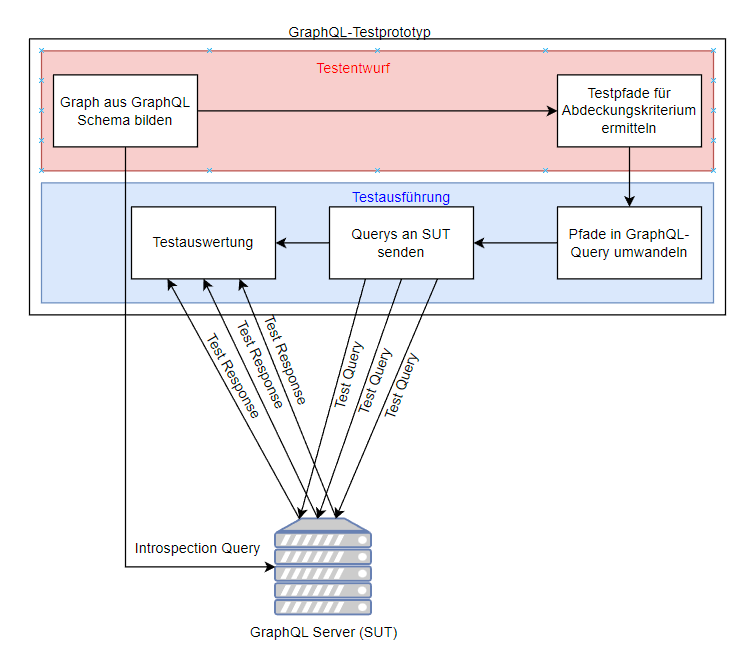
\includegraphics[width=0.75\textwidth,keepaspectratio]{img/fktweiseprototyp}
    \caption{Grober Ablauf des Testprozesses}
    \label{methodeablauf}
\end{figure}

Wie in Abbildung~\ref{methodeablauf} zu sehen, ist der gesamte Testprozess in zwei Teile aufgeteilt.
Einerseits in den Testentwurf, andererseits in die Testausführung.
Der Testentwurf basiert auf den zuvor erarbeiteten Theorien und die Testausführung orientiert sich stark am
Property-based Testing~\cite[vgl. Method]{property-based-testing}.

\section{Testentwurf}
\label{testentw}
Der erste Abschnitt des Testprozesses erarbeitet die Pfadgenerierung nach gewähltem Abdeckungskriterium.
Wie zuvor festgestellt, wird die PrimePfad Abdeckung im Folgenden ermittelt.
Die Methode erlaubt allerdings auch einen Wechsel des Abdeckungskriteriums, da im Endeffekt nur die Pfade für die weiteren Prozesse
genutzt werden können.
Bevor jedoch ein Abdeckungskriterium genutzt werden kann, muss das GraphQL-Schema in einen Graphen übersetzt werden.

\subsection{GraphQL-Schema in Graph abbilden}
\label{schemagraph}

Laut GraphQL-Specification~\cite{graphqlspecification} erlaubt ein GraphQL Server, dass Abfragen über die Schemastruktur des
Servers erlaubt sind~\cite[vgl. 4. Introspection]{graphqlspecification}.
Mithilfe der Introspection-Query~\ref{introspection-query} lässt sich das gesamte Schema eines GraphQL-Servers abrufen.
Die Introspection-Query existiert in verschiedenen Varianten.
Hier wird die exakt gleiche Version genutzt, wie sie auch von~\cite{property-based-testing} verwendet wird.
Ergebnis der Introspection Query ist ein JSON-Objekt mit einer Struktur wie in Listing~\ref{introspec} gezeigt.

\begin{lstlisting}[language=json, caption={Schema-Response},captionpos=b]
    {
        "data": {
            "__schema": {
                "queryType": {},
                "mutationType": {},
                "subscriptionType": {},
                "types": [],
            }
        }
    }
\end{lstlisting}
\label{introspec}

Der Eintrag $queryType$ gibt den Namen des Typens an, der Startpunkt jeder Query ist, so wie in Kapitel~\ref{gqlcov} festgelegt.
Im Eintrag $types$ ist eine Liste aller Typen enthalten, wobei jeder Eintrag der Struktur im Listing~\ref{typstrukt} entspricht.

\begin{lstlisting}[language=json, caption={Type-Field},captionpos=b]
        {
          "kind": "",
          "name": "",
          "description": "",
          "fields": [],
          "inputFields": [],
          "interfaces": [],
          "enumValues": [],
          "possibleTypes": []
        }
\end{lstlisting}
\label{typstrukt}


Um aus dem Schema einen Graphen zu erstellen, werden die Felder $kind$, $name$ und $fields$ benötigt.
Die Angabe $kind$ gibt an, von welchem Typ das Feld ist.
Hierbei gibt es 9 Möglichkeiten, die dieses Feld annehmen kann.

\begin{itemize}
    \item \textbf{ObjectTypeDefinition (OBJECT):} Repräsentiert ein Objekt mit Feldern.
    \item \textbf{ScalarTypeDefinition (SCALAR):} Eingebaute oder benutzerdefinierte Typen wie \texttt{Int}, \texttt{Float}, \texttt{String}, \texttt{Boolean} und \texttt{ID}.
    \item \textbf{InputObjectTypeDefinition (INPUT\_OBJECT):} Erlaubt das Übergeben komplexer Objekte als Argumente.
    \item \textbf{InterfaceTypeDefinition (INTERFACE):} Repräsentiert eine Liste von Feldern, die andere Objekttypen enthalten müssen.
    \item \textbf{UnionTypeDefinition (UNION):} Kann einen von mehreren Arten von Objekttypen repräsentieren.
    \item \textbf{EnumTypeDefinition (ENUM):} Ein Skalartyp, der auf eine bestimmte Liste von Werten beschränkt ist.
    \item \textbf{ListTypeDefinition (LIST):} Repräsentiert eine Liste von Werten eines bestimmten Typs.
    \item \textbf{NonNullTypeDefinition (NON\_NULL):} Ein Modifikator, der angibt, dass der angewandte Typ nicht null sein kann.
    \item \textbf{DirectiveDefinition (DIRECTIVE):} Passt das Verhalten von Feldern oder Typen des Schemas an.
\end{itemize}

Aus allen Feldern des Typen $OBJECT$ kann ein Graph gebildet werden.
Die Menge aller Objekte vom Typ $OBJECT$ ist die Menge aller Knoten des Graphens.
Kanten werden dem Graphen hinzugefügt indem die einzelne Typdefinition näher betrachtet wird.
Wie in $Type-Field$ gesehen, definiert ein Type immer ein Feld $fields$.
In diesem Feld $fields$ verbirgt sich die Informationen aller Kanten, die ausgehend von diesem Knoten sind.
Das Feld $fields$ beeinhaltet Objekte folgender Struktur:

\begin{lstlisting}[language=json, caption={Type-Field},captionpos=b]
            {
              "name": "",
              "description": "",
              "args": [],
              "type": {},
              "isDeprecated": "",
              "deprecationReason": ""
            }
\end{lstlisting}

Wobei für die Ermittlung der Kanten das Feld $type$ besonders wichtig ist.
Das Feld ist nach Schema aus Listing~\ref{typefiel} definiert.

\begin{lstlisting}[language=json, caption={Type-Field},captionpos=b, label={typefiel}]
    {
        "kind": "",
        "name": "",
        "ofType": null
    }
\end{lstlisting}

Wenn der Eintrag $kind$ den Wert $OBJECT$ trägt, so ist klar, dass das hier definierte $OBJECT$ eine Kante zum Knoten $name$ besitzt.

\subsection{PrimePfade ermitteln}
\label{testpfade}

Aus dem zuvor ermittelten Graphen sollen Testpfade ermittelt werden, welche die PrimePfad-Abdeckung erfüllen.
Hierzu wird der in~\cite[Finding Prime Test Paths]{software-testing} vorgestellte Algorithmus genutzt.
Dabei werden zuerst die einfachen Pfade ermittelt und dann gefiltert.
Dies sind Pfade ähnlich zu Definition~\ref{primepfad} mit der Lockerung, dass diese Pfade auch Teilpfad eines längeren Pfads sein können~\cite[vgl. S. 35]{software-testing}.
Der längste einfache Pfad kann maximal so lang sein wie die Anzahl der Knoten des Graphens~\cite[vgl. S.41 ]{software-testing}.
Es wird von jedem Knoten aus expandiert und eine Liste über alle Pfade geführt.
Pfade werden nicht weiter expandiert, wenn diese einen Knoten doppelt enthalten.
Das Endergebnis ist dann eine Liste aller einfachen Pfade.
Diese Liste wird gefiltert, indem alle Pfade, die Teilpfad eines anderen Pfads sind, verworfen werden.
Nach Definition~\ref{primecov} wird so die PrimePfad-Abdeckung erlangt.
Dies folgt, da die Menge der PrimePfade eine echte Teilmenge der einfachen Pfade ist~\cite[vgl. S. 35]{software-testing}.
Mit der Einschränkung von GraphQL, dass valide Queries stets im Query-Knoten starten müssen, muss sichergestellt werden, dass die PrimePfade dort starten.
Um dies umzusetzen, wird festgelegt, dass der kürzeste Weg vom Query Knoten zum Startknoten des PrimePfades zu ermitteln ist und an den PrimePfad anzuhängen,
sodass aus diesem später eine valide Query generiert werden kann.
Es lässt sich also festhalten, dass zuerst die Pfade für eine PrimePfad Abdeckung berechnet werden müssen
und diese dann zu gültigen Testpfaden erweitert werden sollen, sodass sie GraphQL Konventionen einhalten.

\newpage
\section{Testausführung}

Die ermittelten Pfade werden zu validen GraphQL-Queries umgewandelt und dann ausgeführt um den Test zu validieren.
Die Pfadumwandlung in eine valide Query ist noch methodisch stark abweichend zu~\cite{property-based-testing}.
Spätere Schritte, also Test ausführen und auswerten sind methodisch gleich zu~\cite{property-based-testing}.

\subsection{Pfade in Query umwandeln}
\label{pfadquery}

Die Umwandlung eines Pfads in eine Query erfolgt durch die Verwendung der Typinformationen aus dem GraphQL-Schema.
Der Pfad wird beginnend im Query-Knoten abgelaufen.
Das GraphQL-Schema enthält Informationen darüber, welche Informationen nötig sind, um zum nächsten adjazenten Knoten des Pfads zu kommen.
Die Informationen darüber sind im Eintrag $fields$ enthalten, wie in Listing~\ref{typstrukt} gesehen.
Im $fields$ Eintrag steht, ob eine Kante Argumente benötigt und welchen Typ das Rückgabeobjekt hat.
Das Rückgabeobjekt des $fields$ steht dabei aber schon fest, da dieser exakt gleich sein muss mit dem nächsten Knoten des Pfads.
In jedem Schritt der Query-Generierung werden stets alle Felder vom Typ $SCALAR$ hinzugefügt, damit sichergestellt werden kann, dass
der Typ alle Felder implementiert hat.
Je nach Implementierung können durch die Feldauswahl weitere Funktionen abgefragt werden, daher ist alles zu inkludieren.
Felder vom Typ $OBJECT$ werden nur zur Query hinzugefügt, wenn der Typ des $OBJECT$ dem nächsten Knoten entspricht.
Im Allgemeinen lässt sich das Verfahren durch den Pseudocode in Listing~\ref{pfadgen} darstellen. \\

\begin{lstlisting}[caption={Pseudocode für Pfadgenerierung},captionpos=b, label={pfadgen}]
    path = (A , B , ..... , Y)
    query = {}

    while path not empty:
        knoten = pfad.pop()
        ScalarFields = getScalarFields(knoten)
        query.addScalars(ScalarFields)
        edge = pfad.peek()
        args = checkForEdgeArgs(edge)
        query.addArgs(args)
    return query
\end{lstlisting}

Die Argumente, die in einer Query verwendet werden, sind stets nur $SCALAR$ Types und somit einfache Datentypen.
Es gibt verschiedene Arten die Argumentgeneratoren umzusetzen, vorerst werden diese jedoch methodisch exakt wie in~\cite{property-based-testing} umgesetzt.
Dabei wird der Typ des Arguments genutzt, um zufällig ein Argument des entsprechenden Datentyps zu generieren.
Ergebnis des Prozesses ist schließlich eine valide GraphQL-Query.
In einer konkreten Implementierung ist die Syntax von GraphQL zu beachten, diese ist einsehbar in~\cite[2.3 Language Operations]{graphqlspecification}.

\subsection{Queries an Server senden}
\label{testf}

Die generierten Queries stellen die konkreten Tests für den GraphQL-Server dar.
Im Folgenden wird der GraphQL-Server vermehrt SUT (System under Test) genannt.
Eine Auswertung der Tests geschieht, indem alle generierten Queries per HTTP-POST an den GraphQL-Server geschickt werden.
Die gelieferten Antworten sind zu speichern, dies ist analog zu~\cite{property-based-testing}.
Es ist wünschenswert, dass die generierten Queries in einem Testframework abgebildet und gespeichert werden.
Dadurch werden die Tests reproduzierbar und können später verwendet werden, um etwaige Fehlerbehebungen zu verifizieren.

\subsection{Testauswertung}

Die Auswertung der Tests basiert auf denselben Annahmen, wie sie in~\cite{property-based-testing} getroffen wurden.
Dabei werden die HTTP-Codes der Antworten (im folgenden oft Response) und die existierenden Keys in der Response überprüft.
Eine Antwort eines GraphQL-Servers liefert stets einen Statuscode \textbf{200}, wenn kein kritischer Fehler auftrat.
Kritische Fehler sind stets ein Statuscode \textbf{500}~\cite[vgl. 7. Response]{graphqlspecification}.
Daher wird jede Antwort mit einem Code \textbf{500} als gefundener Fehler und fehlerhafter Test betrachtet.
Eine Antwort mit einem Statuscode \textbf{200} kann jedoch auch Fehler aufweisen.
Dies wird ersichtlich durch einen zweiten Haupteintrag $errors$ in einer Antwort, ersichtlich in Listing~\ref{err}.

\begin{lstlisting}[language=GraphQL, label={err}, caption={fehlerhafte Antwort}]
    {
        "data": {}
        "errors": {}
    }
\end{lstlisting}

Die Einträge in $errors$ müssen jedoch manuell geprüft werden, ob es sich um einen wirklichen Programmierfehler handelt oder gewünschtes Verhalten,
da die Zufallsargumente teilweise dafür sorgen, dass Konventionen nicht eingehalten werden können.
Die Zufallsargumente sorgen allerdings auch dafür, dass die errechnete PrimePfad Abdeckung nicht praktisch erreicht wird.
Sehr häufig kommt es vor, dass zufällig generierte Argumente schon in den Anfängen des Pfads nicht passend zu den vorhandenen Daten sind.
Dadurch folgt, dass ein Großteil der Testpfade, die theoretisch eine gute Abdeckung aufweisen, praktisch diese Abdeckung nicht erreicht.
Um messen zu können, ob ein Pfad seine theoretische Abdeckung auch praktisch erreicht, wird eine Abschätzung eingeführt.

\subsubsection{Abschätzung der Pfadlängen}

Mit einer Abschätzung werden die Testergebnisse nicht besser, allerdings können so Informationen darüber gewonnen werden, wie viel
vom getesteten Pfad tatsächlich abgedeckt wurde.
Dadurch lässt sich der Erfolg der Tests besser abschätzen, da so messbar wird, ob die Queries wirklich die Funktionen ausgeführt haben.
Hierzu wird die Pfadlänge des Pfads, der zur Erstellung der Query genutzt wurde, als erwartete Pfadlänge angenommen.
Die Pfadlänge der Antwort wird dann als tatsächliche Pfadlänge genommen.
Der Unterschied zwischen erwarteter und tatsächlicher Pfadlänge ist dann das Auswertungsmerkmal für diesen speziellen Test.
Die Pfadlänge der Response ist die maximale Tiefe der JSON-Response verringert um 1.

\[ \text{Tiefe des Pfades} = \text{Tiefe des JSON-Response-Objekts} - 1 \]

Demnach hat die Response aus Listing~\ref{resp3} eine Tiefe von 2.

\begin{lstlisting}[language=GraphQL, caption={vollständige Response}, label={resp3}]
    {
        "data": {
            "book": {
                id: "1",
                title: "Moby Dick"
                publisher: {
                    id: "1",
                    name: "Testverlag"
                }
            }
        }
    }
\end{lstlisting}

Eine leere Antwort, wie in Listing~\ref{resp4} gezeigt, hat eine Tiefe von 1.

\begin{lstlisting}[language=GraphQL, caption={mangelhafte Response}, label={resp4}]
    {
        "data": {
            "book": null
        }
    }
\end{lstlisting}

Obwohl eine leere Response zulässig ist und nicht direkt auf einen Fehler hindeutet, signalisiert der Unterschied zwischen erwarteter und tatsächlicher Länge,
ob die Query tatsächlich alle Resolver ausgeführt hat oder nur einen Teil davon.
Mithilfe der Abschätzung kann die Qualität der Tests ausgewertet werden.
Hierzu kann die Pfadlänge aller erwarteten Pfade addiert werden.
Das gleiche wird mit den tatsächlichen Pfadlängen gemacht.
Beide Zahlen können dann miteinander in Bezug gesetzt werden, um eine prozentuale Einschätzung zu erlangen, wie viel Prozent der Tests
tatsächlich ausgeführt wurden.
\begin{definition}
    \[ \text{Prozent der tatsächlichen Abdeckung} = \frac{\text{tatsächliche Gesamtpfadlänge}}{\text{erwartete Gesamtpfadlänge}} * 100 \]
\end{definition}

Ein Wert von 100\% ist anzustreben.
Dies würde bedeuten, dass die generierten Tests auch alle Funktionen getestet haben.
In der Praxis wird der Wert jedoch sehr wahrscheinlich darunter liegen.
\\
\\

Abschließend soll erklärt werden, wie es möglich ist, den Wert der tatsächlichen Abdeckung zu erhöhen.
Dies geschieht durch zwei verschiedene Methoden.

\subsubsection{Zufallsgeneratoren der Argumente}
\label{zufallsgen}

Die zuvor vorgestellte Abschätzung liefert einen Hinweis darüber, wie gut die Queries tatsächlich getestet wurden.
Ein Ansatz, der die Queries eine bessere tatsächliche Abdeckung erreichen lässt, ist das Anpassen der Generatoren für die Argumente.
Bei der in Kapitel~\ref{pfadquery} vorgestellten Methode werden Argumente komplett zufällig für den zugrundeliegenden Datentyp erstellt.
Dies bedeutet, dass zum Beispiel der Type $ID$ als String gewertet wird.
Eine $ID$ unterliegt jedoch in den allermeisten Implementierungen bestimmten Konventionen.
So wäre ein Generator für zufällige Strings nicht in der Lage, solche Konventionen zuverlässig abzubilden.
Ein Anpassen des Argumentgenerators für die $ID$ an die verwendete Konvention des SUT hilft dabei, dass signifikant bessere Ergebnisse erzeugt werden.
Alternativ kann auch eine Liste aller existenten IDs angegeben sein und zufällig ein Element ausgewählt werden.
Die Anpassung der Argumentgeneratoren an die zugrundeliegenden Daten ist höchst spezifisch und daher kann keine allgemeine
Vorgehensweise ermittelt werden.
Ziel der Anpassung ist es, dass die Chance erhöht wird, dass Argumente zufällig generiert werden, die dann tatsächlich zu den zugrunde liegenden Daten passen.

\subsubsection{Anzahl der Queries}

Die Wahrscheinlichkeit, passende Argumente zu generieren, steigt mit der Anzahl an generierten Queries.
Wird die Anzahl an generierten Queries pro Pfad erhöht, so steigt auch die Wahrscheinlichkeit, dass zumindest ein Pfad eine gute Abdeckung erreicht.
Hierfür muss die Methode aus Kapitel~\ref{pfadquery} so oft wie gewünscht wiederholt werden.
In jeder Generierung muss jedoch das Ergebnis sein, dass verschiedene Argumente für die Query generiert wurden.
Zusammen mit den angepassten Argumentgeneratoren kann so die zufallsbasierte Argumentgeneration begrenzt werden
und es ist wahrscheinlicher, dass gute Tests entstehen.


\section{Zusammenfassung der Methode}

Die eben entwickelte Methode funktioniert so wie in Abbildung~\ref{methodeablauf} gezeigt.
Teile der Methode bedienen sich an Methoden die in~\cite{property-based-testing} eingeführt wurden.
Der komplette Prozess der Testgenerierung wurde in der hier entwickelten Methode jedoch verändert.
So wurde die Graphstruktur von GraphQL genutzt, um aus dieser Testpfade zu generieren, die dann in GraphQL-Queries umgewandelt werden.
Auf diese Weise war es möglich, die Limitierung des Rekursionslimits vom \textit{Property-based Testing} zu beseitigen.
In der Testauswertung wurde sich stark am \textit{Property-based Testing} orientiert.
Die Einführung der erwarteten Pfadlänge gegenüber der tatsächlichen Pfadlänge ist ein neuer Ansatz, der die Qualität der zu testenden Queries
messbar macht.
Das fehlt im \textit{Property-based Testing} .
\\


Im Folgenden soll die entwickelte Methode in einem Prototypen umgesetzt werden.
Dieser Prototyp soll dann in Experimenten zeigen, dass die entwickelte Methode in der Lage ist, Fehler in GraphQL-APIs zu finden.
Ein Vergleich mit dem Prototypen von \textit{Property-based Testing} soll zeigen, ob die Methode Verbesserungen bringt.








  \chapter{Testautomatisierung}

Hi


  \chapter{Praxis}

Nach der Einführung der Methode im vorherigen Kapitel soll nun der entwickelte Prototyp umfassend erklärt werden.
Der entwickelte Prototyp lässt sich unter \href{https://github.com/gernhard1337/graphql-primepath-tester} finden und testen.
Eine erklärende Readme existiert im Root-Verzeichnis.
Vorraussetzungen zum Ausführen der Anwendung ist Python und diverse Dritt-Bibliotheken die in der Readme vermerkt sind.

\section{Tool- / Dependencyauswahl}
Um die vorgestellte Methode umzusetzen war insbesondere wichtig, dass eine einfache und mächtige Bibliothek für die Definition und Bearbeitung
von Graphen zur Verfügung steht.
Die erste Wahl fiel hierbei auf NetworkX, eine Graphenbibliothek in Python.
Sie wurde ausgewählt da der Ersteller schon einige Erfahrungen mit dieser Bibliothek hat und somit eine effiziente Umsetzung möglich war.
Dadurch, dass diese Bibliothek als Grundlage gewählt wurde hat sich die Programmiersprache Python schnell ergeben.
Im folgenden werden einige weitere benutzte Bibliotheken kurz vorgestellt sodass der Applikationsstack übersichtlich wird.
Wir werden auch auf NetworkX und seine Features eingehen.
Es werden nicht alle Bibliotheken eine Berücksichtigung finden sondern nur diese, die einen signifikanten Einfluss auf das Programm haben und besonders herausstechen.

\subsection{NetworkX}

NetworkX ist eine Python-Biblitohek für \textit{Erstellung, Manipulation und Untersuchung der Struktur, Dynamik und Funktionen komplexer Netzwerke}~\cite[vgl. Startseite]{networkx}
Mit einer Star-Anzahl von \textit{12.8k}\cite{networkxgithub} auf GitHub ist networkX eine sehr beliebte Bibliothek.
NetworkX ist die ideale Wahl um Graphen zu erstellen für unseren Use-Case denn es nimmt jeden möglichen Datentypen als Wert für einen Knoten und Kante.
Wir können also sehr simpel Graphen definieren.
Für das simple Beispiel von Author, Book, Publisher und deren Verbindungen benötigen wir nur folgende Zeilen:

\begin{lstlisting}[language=Python]
    import networkx as nx

    G = nx.Graph()
    G.add_edge("Query", "Book", "book")
    G.add_edge("Query", "Author", "author")
    G.add_edge("Query", "Publisher", "publisher")

    G.add_edge("Publisher", "Book", "book")
    G.add_edge("Book", "Publisher", "publisher")

    G.add_edge("Book", "Author", "author")
    G.add_edge("Author", "Book", "book")
\end{lstlisting}

Diese wenigen Zeilen reichen aus um unseren Graphen mit allen Knoten und Kanten zu definieren.
Wie zuvor eingeführt existiert auch das Kantengewicht, dass der Feldbezeichner eines Types ist.
Auf diesem Graphen können wir dann diverse Algorithmen ablaufen lassen.
Diverse Hilfsfunktionen helfen dabei eine effiziente Programmierung zu erlangen.
Hierbei seien insbesondere folgende Hilfsfunktionen genannt:

\subsubsection{draw}
    \begin{lstlisting}[language=Python]
        nx.draw(G, with_labels=True)
    \end{lstlisting}

Zeichnet einem den erstellten Graphen in ein beliebiges Format.
So fällt es einfach große Graphen darzustellen.

\subsubsection{shortest\_path}
    \begin{lstlisting}[language=Python]
        shortest_path = nx.shortest_path(G, Node1, Node5)
    \end{lstlisting}

Die Funktion $shortest\_path$ gibt eine Liste von Kanten zurück, die den kürzesten Weg zwischen zwei
Knoten angibt.

\subsubsection{neighbors}
    \begin{lstlisting}[language=Python]
        G.neighbors(Node)
    \end{lstlisting}
Diese Funktion liefert alle Nachbarn eines Knotens.
In unserem Kontext eine sehr wichtige Funktion wie wir später noch sehen werden.

\subsection{Faker}
Die gewählte Datengenerierungsbibliothek ist \textit{Faker}\cite{fakergithub}.
Mit \textit{16k}\cite{fakergithub} Sternen auf GitHub ist Faker eine noch beliebtere Bilbiothek als NetworkX.
Faker ist eine Bilbiothek die es sehr einfach macht Daten zu generieren.
Da wir im Kontext von GraphQL Argumenten nur sehr einfache Datentypen als Argumente benötigen reicht uns diese
Bibliothek komplett aus da sie es schafft uns schnell und unkompliziert Daten in genau dem Format zu generieren wie wir sie brauchen.
Angenommen wir benötigen einen String der 10 Zeichen lang ist, so reicht eine Zeile:

\begin{lstlisting}[language=Python]
        random_string = fake.pystr(min_chars=10, max_chars=10)
\end{lstlisting}

Selbiges falls wir eine Zufallszahl benötigen zwischen 1 bis 1000

\begin{lstlisting}[language=Python]
        random_number = fake.random_int(min=1, max=1000)
\end{lstlisting}

Diese Schema des Einzeilers zieht sich für alle simplen $SCALAR$ Types in GraphQL.
Daher fällt die Wahl für die Datengenerierung auf diese Bibliothek.

\subsection{PyTest}

Nicht zwingend notwendig ist ein Testframework.
Allerdings soll unsere Implementation der Methode Tests erstellen sodass diese zu einem späteren Zeitpunk erneut ausgeführt werden können.
Somit können wir z.B. überprüfen ob eine Korrektur des Servercodes eine Verbesserung gebracht hat.
Hierfür wollen wir die Tests mithilfe eines Testframeworks erstellen.
Die Wahl hierfür fiel dabei auf PyTest.
PyTest ist ein Testframework für Python welches eine simple und einfache Testdefinition ermöglicht.
Ein Test für eine einfache Funktion $inc$ kann mit $test\_inc$ umgesetzt werden.

\begin{lstlisting}[language=Python]
    def inc(x):
        return x + 1

    def test_inc():
        assert inc(3) == 5
\end{lstlisting}

Dies reicht schon vollkommen aus für unsere Testentwicklung daher wurde sich für diese Bibliothek entschieden.

\section{Umsetzung der Methode}

Für die Umsetzung der Methode werden wir durch die einzelnen Teile des Codes gehen und die jeweiligen Stellen erklären die
einzelne Schritte der entwickelten Methode durchgehen.
Hierbei gehen wir chronologisch in den einzelnen Schritten vor so wie in der Methode definiert.

\subsection{Schema in Graph abbilden}

Wie in der Vorstellung der Methode unter $6.1$ bilden wir das GraphQL-Schema in einem Graphen ab.
Hierfür nutzen wir die zuvor erwähnt Python Graphbibliothek NetworkX.
Um die Informationen zu erlangen die für die Bildung des Graphens wichtig sind führen wir die Introspection-Query \ref{introspection-query}
aus.
Das Ergebnis ist dann das vollständige GraphQL-Schema der API.
Hierbei sei angemerkt, dass einige GraphQL APIs so eine Introspection-Query verbieten, sei es einerseits durch direktes verbieten oder ein Tiefenlimit in den Querys.
Egal was hierbei der Fall ist, die zu testende API muss unsere Introspection-Query \ref{introspection-query} unterstützen.
Die Query wird mit einem simplen HTTP-POST an die zu testende URL gesendet.

\begin{lstlisting}[language=Python]
    r = requests.post(testUrl, json={'query': queries.introspection_query})
    json_data = json.loads(r.text)
    with open('schema.json', 'w') as f:
        json.dump(json_data, f)
\end{lstlisting}

Und die Response wird als JSON-Objekt in $json\_data$ gespeichert.
Zudem speichern wir das JSON-Objekt der aktuellen API auch ab damit diese später gegebenenfalls untersucht werden kann.
Es wurde ein Modul $Graphhandler$ entwickelt, dass verschiedene Graphoperationen für einen Übernimmt.
Im Graphhandler ist eine Funktion $buildGraph$ definiert.
Diese generiert einen Graphen von einem gegebenen Startknoten, einem leeren Graphen und dem Schema.
Hierbei werden nur erreichbare Knoten von Startknoten berücksichtigt.
Setzt man den Startknoten auf den Knoten $Query$ so inkludieren wir auf diese Weise nur alle erreichbaren Teile
des Graphens ausgehend von $Query$.
Dies ist insofern sinnvoll da andere Typen, wenn sie nicht von $Query$ aus erreichbar sind, nicht Teil des Testraumes wären da diese
in keiner validen Anfrage vorkommen können.
Die Funktion, die den Graphen generiert sieht wie folgt aus:

\begin{lstlisting}[language=Python]
def buildGraph(graph, type_name, type_dict):
    if type_name.startswith(nonSchemaTypePrefix) or type_name in baseDatatypes:
        pass
    else:
        for adjacentNode in type_dict[type_name]['fields']:
            if graph.has_edge(type_name, adjacentNode['type']['name']):
                return
            else:
                if adjacentNode['type']['name'] and adjacentNode['type']['name'] not in baseDatatypes:
                    graph.add_edge(type_name, adjacentNode['type']['name'])
                    graph[type_name][adjacentNode['type']['name']]["data"] = adjacentNode
                    buildGraph(graph, adjacentNode['type']['name'], type_dict)
                if adjacentNode['type']['kind'] == 'LIST' and adjacentNode['type']['ofType']['name'] not in baseDatatypes:
                    graph.add_edge(type_name, adjacentNode['type']['ofType']['name'])
                    graph[type_name][adjacentNode['type']['ofType']['name']]["data"] = adjacentNode
                    buildGraph(graph, adjacentNode['type']['ofType']['name'], type_dict)

\end{lstlisting}

Die Funktion buildGraph arbeitet rekursiv.
Vom Startknoten (im Allgemeinen $Query$) aus rufen wir die Funktion auf allen Folgeknoten von Query auf.
Dies sind alle Knoten die den Type $OBJECT$ besitzen und nicht mit einem $\_\_$ beginnen oder ein Basisdatentyp sind.
GraphQL kann eigene Objekte definieren welche mit $\_\_$ starten, diese schließen wir explizit aus genau wie alle $SCALAR$ Types.
Jeder Knoten definiert nun in seinem $fields$ Eintrag zu welchen Feldern er Beziehungen hat.
Hierbei muss unterschieden werden, dass ein Eintrag entweder vom Type $OBJECT$ oder $LIST$ sein kann, um zulässig zu sein.
Sollte es sich um einen $LIST$ Eintrag handeln müssen wir prüfen von welchem Type die $LIST$ ist.
Wenn ein Knoten nun unsere Bedingungen erfüllt, so wird dieser dem Graphen hinzugefügt und auf ihm selbst wird $buildGraph$ ausgeführt.
So erlangen wir die gesamte Graphstruktur da ausgehend von Query jeder erreichbare Knoten hinzugefügt wird und dann von diesem Knoten eben wieder alle erreichbaren Knoten
hinzugefügt werden.

\subsection{Pfade aus Graph bilden}

Der Graphhandler implementiert verschiedene Coveragekriterien.
Das Tool benötigt eine Liste $paths$ die aus Kanten besteht.

\begin{lstlisting}[language=Python]
paths = graphhandler.generate_prime_paths("Query", graph)
\end{lstlisting}

Eine Funktion $generate\_CoverPaths$ kann jedes erdenkliche Coveragekriterium umsetzen.
In unserem Fall sind es insbesondere PrimePaths, umgesetzt durch die Funktion $generare\_prime\_paths("Query", graph)$.
Diese Funktion ermittelt die PrimePaths ausgehend vom Startknoten $Query$ im definierten Graphen.
Will man ein anderes Coveragekriterium umsetzen, so muss die Funktion $generate\_CoverPaths$ eine Liste der Kanten zurückgeben
die dem Coveragekriterium entsprechend den Graphen überdecken.
Die Generierung der PrimePaths sehen wir uns nun noch genauer an.
Wir starten mit der Funktion $generare\_prime\_paths()$.
Diese bekommt einen Startknoten und einen Graphen.
Sie gibt dann die Liste der Pfade genau wie zuvor spezifiziert zurück.

\begin{lstlisting}[language=Python]
def generate_prime_paths(startknoten, g):
    pfadliste = []
    generate_paths(startknoten, [], pfadliste, g)
    return pfadliste
\end{lstlisting}

Es wird die Funktion $generate\_paths$ aufgerufen wobei generate\_paths sich immer wieder rekursiv selbst aufruft wenn die Nachfolger des Knotens
noch nicht im Pfad sind. So werden Kreise verhindert, alle Pfade die so erzeugt werden sind SimplePaths.

\begin{lstlisting}[language=Python]
def generate_paths(n, path, pathList, g):
    path.append(n)
    for m in g.successors(n):  # successors gibt die Nachfolger wieder
        if m not in path:
            generate_paths(m, copy.deepcopy(path), pathList, g)
    if is_prime_path(path, pathList):
        pathList.append(path)
\end{lstlisting}

Sollte ein SimplePath dann ein PrimePath sein so wird dieser zurückgegeben.
Ein Pfad ist ein Prime-Pfad, wenn er kein Teil eines bereits existierenden Pfades ist und keine Kreise enthält.
Diese drei hier vorgestellten Funktionen setzen den Pseudocode aus $6.3.2$ um

\begin{lstlisting}[language=Python]
def is_prime_path(new_path, pathList):
    for exisiting_paths in pathList:
        if is_subpath(new_path, exisiting_paths):
            return False
    return True
\end{lstlisting}





% Das wird in der Implementierung teilweise schon anders gemacht und wird vielleicht nicht gebraucht.
\subsection{Coveragepfade ermitteln (maybe remove - TODO)}


\subsection{Querys aus Pfad ermitteln}
\subsection{Test ausführen / Testfile generieren}
\subsection{Testauswertung}

\newpage
\section{Zusammenfassung der Implementation}

Die entwickelte Methode lässt sich in folgendem Sequenzdiagramm gut abbilden:

\begin{center}
    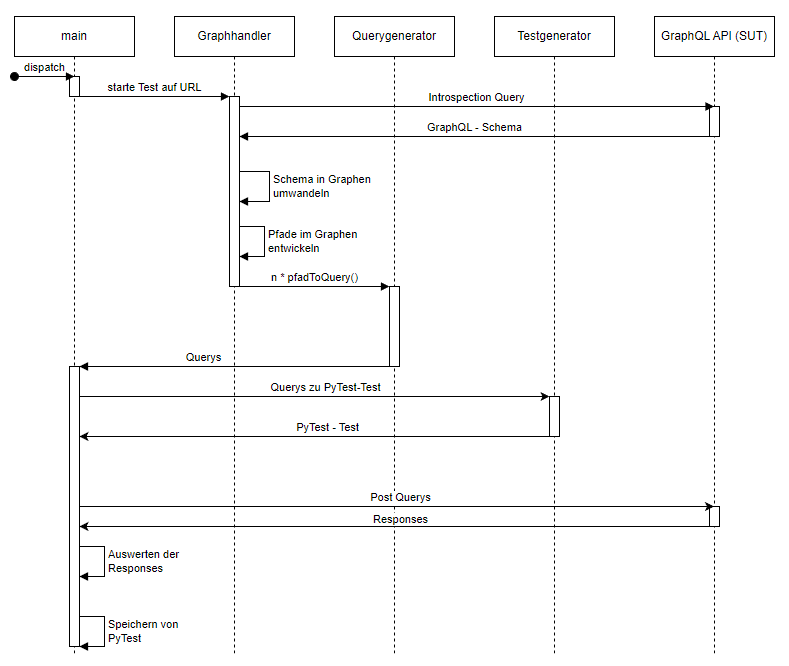
\includegraphics[width=\textwidth,height=\textheight,keepaspectratio]{img/sequenz}
\end{center}







  %Schluss
  \chapter{Zukünftige Arbeit}
\label{futurework}

Einige bereits angesprochene Punkte bieten Möglichkeiten für eine Erweiterung der hier geleisteten Arbeit.
Während in dieser Arbeit ein erheblicher Beitrag zur theoretischen Testabdeckung von GraphQL-APIs geleistet wurde,
so ist nicht garantiert, dass die entwickelten Tests tatsächlich die ermittelte Abdeckung erreichen.
Dies folgert sich aus der zufälligen Argumentgenerierung in den einzelnen Queries.
Ziel ist es nun, den Zufall möglichst weit zu begrenzen oder aber die erlangten Ergebnisse sinnvoller zu nutzen.
Im Folgenden werden zwei Ansätze vorgestellt, die das Potenzial haben, eine praktische Testausführung zuverlässiger und präziser machen zu können.
Ziel von weiterführenden Arbeiten sollte es sein, dass die tatsächliche Pfadabdeckung sich der theoretischen Pfadabdeckung annähert.

\section{BlackBox-Testing in WhiteBox-Testing umwandeln}

Das Testsystem hat im BlackBox-Testing keinerlei Informationen über das SUT und Testgenerierung auf GraphQL-APIs ohne die Argumentgeneratoren anzupassen,
führt häufig dazu, dass die generierten Daten nicht zum SUT passen.
Im experimentellen Ansatz wurde der BlackBox Ansatz abgeschwächt und zu einem GreyBox-Ansatz verändert, indem die Argumentgeneratoren mit Domänenwissen an das jeweilige SUT angepasst wurden,
sodass die zufällige Argumentgenerierung mit höherer Wahrscheinlichkeit ein Argument liefert, das dem Test eine bessere, tatsächliche Abdeckung liefert.
Ideal wäre nun, dass die Testgenerierung auf einem WhiteBox-Ansatz basiert.
Hierdurch ist spezifisches Domänenwissen über das SUT vorhanden, insbesondere dadurch, dass die zugrundeliegenden Daten, Datenstruktur, Programmcode analysierbar sind.
Durch einen White-Box Ansatz wäre es möglich, die Argumentgeneratoren automatisiert anzupassen, sodass sich diese am Schema und den zugrunde-liegenden Daten orientieren.
Außerdem wäre eine Code-Analyse möglich, die dazu führen kann, dass Testfälle noch präziser und exakter Fehler finden.
Die vom Prototypen generierten Testpfade können hierbei weiterhin als Basis dienen, um eine gute Abdeckung sicherzustellen.
Mit optimierten Argumentgeneratoren sollte es möglich sein, die tatsächliche Pfadabdeckung stark zu erhöhen.

\section{Adaptive Generierung}

Die aktuelle Testgenerierung geschieht in einzelnen Phasen.
Es werden erst aus einem Graphen die Pfade generiert, hieraus werden Tests erzeugt und diese werden dann an das SUT gestellt und ausgewertet.
Dabei werden sämtliche Argumente sofort generiert.
Eine adaptive Testgenerierung wäre denkbar, sodass aus einem Testpfad die Query nur in Teilen erstellt wird.
Dabei wird ein Testpfad erst weiter in der Query abgedeckt, wenn ein Argumentgenerator ein Ergebnis zurückliefert, dass die Pfadlänge tatsächlich erhöht und somit signalisiert, dass der zugrundeliegende Test tatsächlich ausgeführt wird.
Eine solche Methode könnte nach dem Ablauf, wie in Abbildung~\ref{adaptive} dargestellt, funktionieren.
Es werden dabei Queries mit Zufallsargumenten erstellt, die einen Teilpfad des Testpfads bilden und erst wenn der Teilpfad des Testpfads tatsächlich abgedeckt ist, wird mit dem nächsten adjazenten Knoten fortgefahren,
sodass die tatsächliche Pfadabdeckung mit der theoretischen Pfadabdeckung übereinstimmt.

\begin{figure}[H]
    \begin{center}
        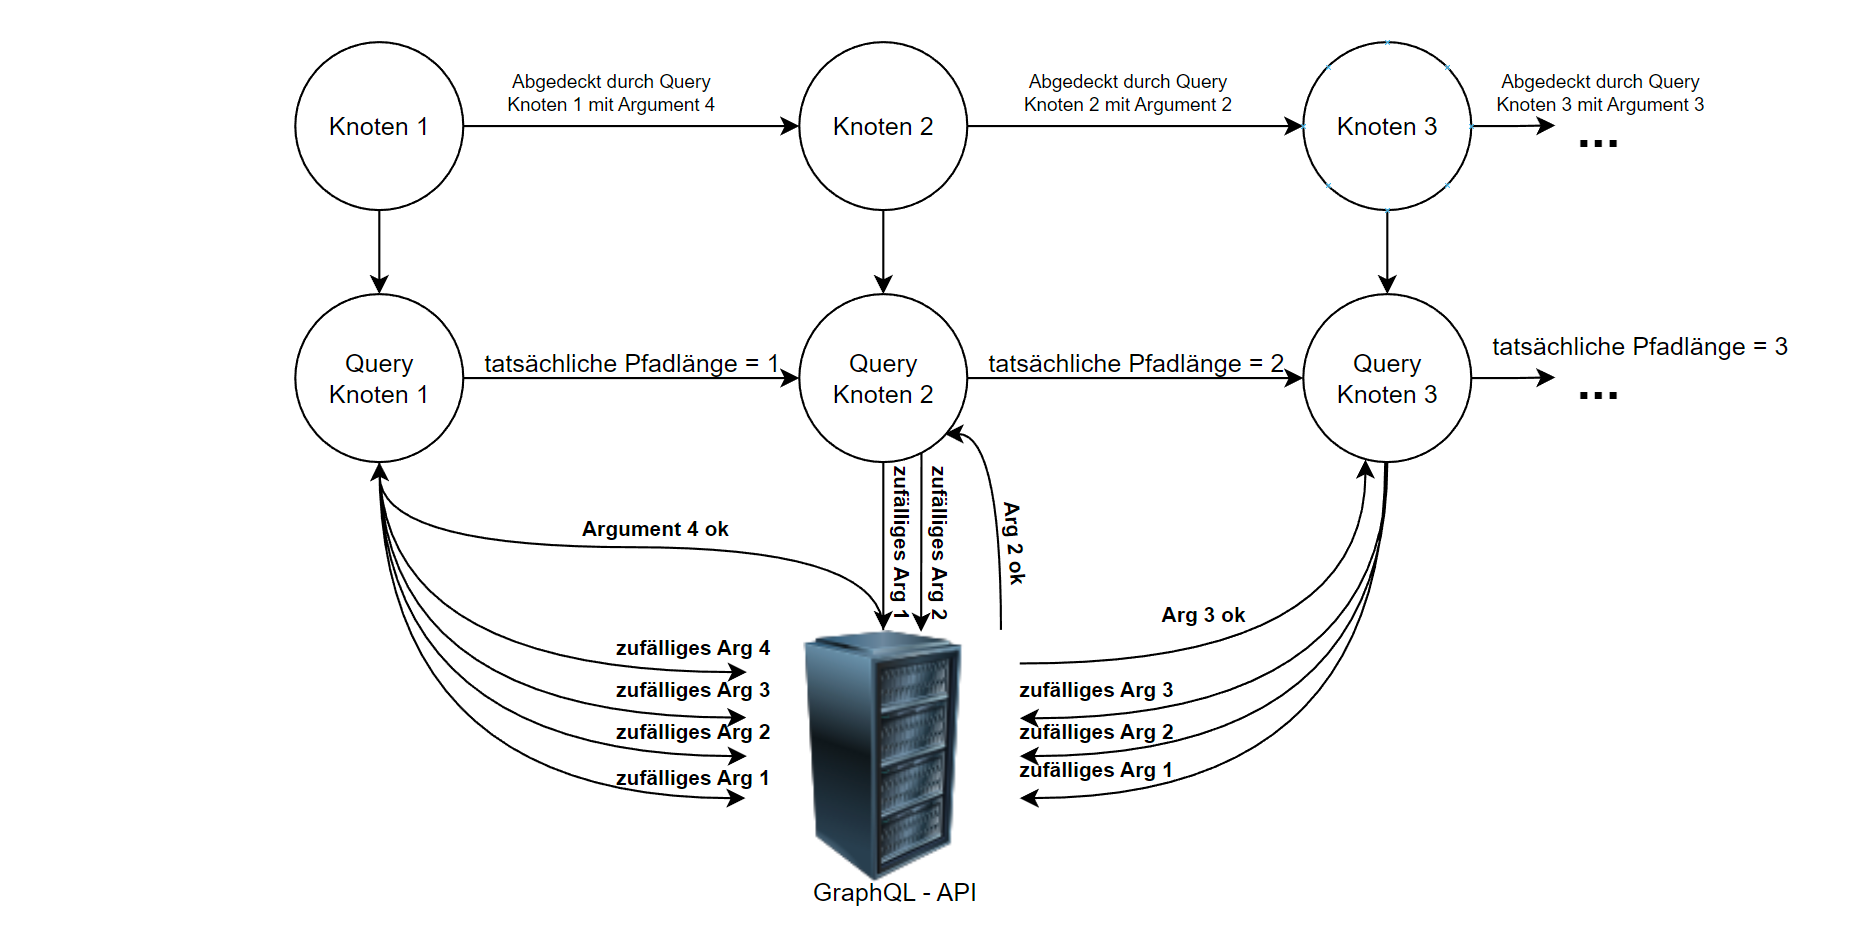
\includegraphics[width=\textwidth,keepaspectratio]{img/ablauffuturework}
    \end{center}
    \caption{Beispielablauf einer adaptiven Generierung}
    \label{adaptive}
\end{figure}

Mögliche Limitierungen wären hierbei jedoch, dass ein Pfad niemals seine gewünschte Pfadlänge erreicht, weil zum Beispiel Daten für den Pfad fehlen und somit jedes Argument unzureichend ist.
Denkbar wäre auch, dass Argumentgeneratoren nicht in der Lage sind, passende Daten zu erzeugen.
Es wären Strategien zu entwickeln, die sicherstellen, dass solche Limitierungen korrekt behandelt werden.
Mit einer solchen Query-Generierung ist eine Steigerung der tatsächlichen Pfadabdeckung möglich und gleichzeitig kann das erlangte Wissen in anderen Pfaden genutzt werden, um die Argumentgenerierung zu vereinfachen.





  \chapter{Fazit}
\label{fazit}

Die Behauptung, dass die Methode des \textit{Property-based Testings} um einen besseren Pfadfindungsalgorithmus als ein simples, zufälliges, begrenztes Raten verbessert werden kann, hat sich als wahr herausgestellt.
Indem ein theoretischer Rahmen geschaffen wurde, war es möglich, Graphabdeckungskriterien zu nutzen, um Tests für GraphQL automatisiert zu generieren.
Die entwickelten Methoden liefern eine gute Grundlage, um das automatisierte Testen von GraphQL weiter voranzutreiben.
Final entstand dann daraus ein Prototyp, der fähig ist, Fehler in GraphQL-APIs zu finden.
Dies wurde an zwei Beispielen gezeigt und nachgewiesen, indem Fehler gefunden werden konnten.
Es wurden Schwachstellen offengelegt und Ansätze entwickelt, die zur Weiterarbeit anregen.
Verwandte Arbeiten wurden betrachtet und dabei konnte festgestellt werden, dass ein Ansatz wie in dieser Arbeit vorher noch nicht betrachtet wurde.
Generell lässt sich sagen, dass GraphQL eine berechtigterweise stetig wachsende Technologie ist und Arbeiten wie diese hier
dazu beitragen, dass die Popularität von GraphQL wächst, da die bisherigen Nachteile von GraphQL gegenüber REST so stückweise aufgelöst werden
und die großen Vorteile erkennbar werden.





  %Anhang
  \backmatter % kennzeichnet den hinteren Teil der Arbeit
  %! Author = Tom
\chapter{Glossar}

Im Text werden einige Fachbegriffe genutzt. Hier findet sich deren Erklärung

\begin{description}
    \item[Begriff] Erklärung
    \item[IEEE/ACM] Ein Journal über Transaktionen in Netzwerken das regelmäßig Konferenzen veranstaltet
    \item[HTTP] HyperTextTransferProtocoll ist ein Übertragunsprotokoll für Datenübertragung
    \item[HTTP-Request] Ist eine Anfrage zum zusenden von Daten
    \item[API] Application Programmable Interface ist eine Schnittstelle wie Systeme miteinander kommunizieren
    \item[REST] Ein Architekturdesign für APIs
    \item[GraphQL] Eine Abfragesprache für APIs die den GraphQL Standard implementieren
    \item[Overfetch] Das Abfrgaen von zu vielen Informationen
    \item[Underfetch] Das Abfragen von zu wenigen Informationen
    \item[SUT] System under Test - ist eine Kurzform für das System, dass es zu testen gilt
    \item[IoT] Internet of Things - meint die Verknüpfung von diversen Geräten mit dem Internet
\end{description}


  \appendix % Anhang

  \cleardoublepage
  \addcontentsline{toc}{chapter}{Literaturverzeichnis}
  %\nocite{*}  % Hier das Kommentarzeichen entfernen, um alle Quellen auszugeben.
  \printbibliography[title={Literaturverzeichnis}]  % Generiert das Literaturverzeichnis

  \vfill
  \begin{center}
   \emph{Onlineressourcen wurden im Juli 2021 auf ihre Verfügbarkeit hin überprüft.}
  \end{center}

\end{document}
